\documentclass[11pt,a4paper]{article}
\usepackage[utf8]{inputenc}
\usepackage[T1]{fontenc}
\usepackage{lmodern}
\usepackage[top=2.15cm,bottom=2.15cm,left=2.25cm,right=2.25cm]{geometry}
\usepackage{amsmath,amssymb,graphicx,booktabs,longtable,array,xcolor}
\definecolor{Brown}{HTML}{A5644E}
\definecolor{Dark}{HTML}{4E3B30}
\definecolor{Blue}{HTML}{2F5D8C}
\definecolor{Beige}{HTML}{F2E8E1}
\usepackage[unicode=true,colorlinks=true,linkcolor=Brown,citecolor=Brown,urlcolor=Blue]{hyperref}
\hypersetup{pdftitle={Depresiasi Rupiah dan Neraca Perdagangan Indonesia},pdfauthor={Tio},pdfsubject={Naskah kerja hasil ARDL dan NARDL berbasis HS-6}}
\renewcommand{\contentsname}{Daftar isi}
\renewcommand{\figurename}{Gambar}
\renewcommand{\tablename}{Tabel}
\renewcommand{\refname}{Daftar pustaka}
\setlength{\parindent}{1.25em}
\setlength{\parskip}{0.32em}
\linespread{1.12}
\setlength{\emergencystretch}{2.5em}
\setcounter{tocdepth}{2}
\setcounter{topnumber}{3}
\setcounter{totalnumber}{4}
\renewcommand{\topfraction}{.9}
\renewcommand{\textfraction}{.08}
\renewcommand{\floatpagefraction}{.65}
\newcommand{\WorldExports}{282,91}
\newcommand{\WorldImports}{241,86}
\newcommand{\WorldNet}{41,05}
\newcommand{\CommodityShare}{51,1}
\newcommand{\ManufacturingShare}{47,1}
\newcommand{\AusBeta}{3,3560}
\newcommand{\AusResponse}{31,99}
\newcommand{\AusRatioPct}{37,69}
\newcommand{\AusBetaMath}{3{,}3560}
\newcommand{\AusResponseMath}{31{,}99}
\newcommand{\readingbox}[1]{\par\medskip\noindent\fcolorbox{Brown}{Beige}{\parbox{\dimexpr\linewidth-2\fboxsep-2\fboxrule}{#1}}\par\medskip}
\begin{document}
\begin{titlepage}\centering
\vspace*{1.1cm}
{\sffamily\color{Brown}\large NASKAH KERJA PENELITIAN\par}
\vspace{1.0cm}
{\sffamily\bfseries\color{Dark}\LARGE Depresiasi Rupiah dan\\[.25em]Neraca Perdagangan Indonesia\par}
\vspace{.6cm}
{\large Bukti ARDL dan NARDL pada perdagangan agregat,\\sepuluh mitra, dan kelompok barang berbasis HS-6\par}
\vspace{1cm}{\large Tio\par}
{\normalsize Versi hasil estimasi: 17 November 2026\par}
\vfill
\begin{minipage}{.88\textwidth}
\readingbox{\textbf{Cakupan.} Seluruh ekspor dan impor adalah milik Indonesia. Istilah \emph{seluruh dunia} menunjukkan seluruh negara mitra Indonesia. HS-6 dipakai membentuk tujuh kelompok; estimasi setiap kode HS-6 secara terpisah belum dilakukan.}
\medskip
Naskah ini menjelaskan hasil yang telah dijalankan di Stata, dengan pembahasan yang lebih panjang daripada presentasi. Statusnya adalah naskah kerja untuk pembelajaran dan pengembangan penelitian, belum artikel jurnal yang telah melalui penelaahan sejawat. Angka, grafik, dan lampiran ditarik dari hasil yang sama dengan PPT; tidak dilakukan estimasi ulang saat menyusun dokumen.
\end{minipage}\vspace{.8cm}
\end{titlepage}
\pagenumbering{roman}
\section*{Abstrak}\addcontentsline{toc}{section}{Abstrak}
Penelitian ini menelaah apakah depresiasi riil rupiah berkaitan dengan perbaikan neraca perdagangan Indonesia secara seragam. Nilai perdagangan bulanan HS-6 Januari 2006--Agustus 2026 diagregasi menjadi kuartal lengkap dan dipadukan dengan kurs riil, indeks harga, serta level PDB riil. Cakupannya adalah perdagangan Indonesia dengan seluruh negara, sepuluh mitra, dan tujuh kelompok barang. Sebanyak 176 model utama ARDL/NARDL dan 340 sensitivitas telah diestimasi di Stata. Outcome adalah log rasio impor terhadap ekspor, sehingga hasil tidak memisahkan respons ekspor dari respons impor. Pada model utama, 95 spesifikasi menolak tidak adanya hubungan level menurut F dan t bounds; 62 memenuhi syarat level tambahan, dan 28 sekaligus memenuhi penyaringan diagnostik yang digunakan. Agregat Indonesia belum memberi dukungan hubungan level yang kuat pada taraf lima persen. Australia dan Malaysia mempunyai dukungan lebih baik pada NARDL bilateral, tetapi signifikansi Malaysia melemah setelah koreksi pengujian berganda. ARDL komoditas total serta energi/tambang mengarah pada pemburukan saat depresiasi, sedangkan NARDL belum mengonfirmasi hubungan yang sama kuat. Pola J terlihat pada sebagian estimasi titik, dengan dukungan interval dan kelayakan model yang lebih terbatas. Hasil memperlihatkan heterogenitas dan ketergantungan pada spesifikasi, bukan pembuktian kausal bahwa depresiasi selalu merugikan atau bahwa komoditas pasti tidak sensitif terhadap kurs.

\noindent\textbf{Kata kunci:} Indonesia; neraca perdagangan; depresiasi riil; J-curve; ARDL; NARDL; komoditas; HS-6.

\section*{Cara membaca naskah}\addcontentsline{toc}{section}{Cara membaca naskah}
Bagian awal menguraikan pertanyaan ekonomi, definisi data dan konstruksi model. Hasil bergerak dari agregat Indonesia ke pasangan bilateral dan kelompok barang. Pembaca yang ingin memahami tanda koefisien sebaiknya membaca Bagian~\ref{sec:methods} sebelum menilai grafik. Bagian~\ref{sec:diagnostics} membahas diagnostik, sensitivitas dan perbedaan antara pola titik dengan dukungan statistik. Lampiran mempertahankan seluruh 516 estimasi dalam bentuk ringkas.

Kode \texttt{WLD} adalah kode mitra agregat, bukan negara pelapor. Negara pelapor tetap Indonesia. Status \texttt{L} dan \texttt{L+D} adalah ringkasan penyaringan operasional, bukan sertifikat kebenaran model. Probabilitas koefisien dan interval bersifat nominal sesudah seleksi AIC.

\clearpage\tableofcontents
\clearpage\pagenumbering{arabic}
\section{Pendahuluan}\label{sec:intro}
\subsection{Pertanyaan ekonomi}
Depresiasi sering dihubungkan dengan peningkatan daya saing karena harga barang domestik menjadi relatif lebih murah bagi pembeli asing. Penjelasan tersebut merupakan titik awal yang berguna, tetapi belum menetapkan arah perubahan neraca perdagangan. Nilai ekspor dan impor juga bergantung pada harga internasional, permintaan, kemampuan produksi, dan waktu penyesuaian. Respons suatu barang atau pasar dapat berbeda dari respons agregat. Penelitian ini menanyakan sejauh mana perbaikan yang diharapkan terlihat pada perdagangan Indonesia, dan apakah kesimpulannya bertahan ketika arah perubahan kurs serta komposisi barang dipisahkan.

Motivasi awal berkaitan dengan besarnya peran komoditas dalam ekspor Indonesia. Pada rincian HS-6 yang digunakan, komoditas yang dapat dipetakan secara konservatif mencakup \CommodityShare\% nilai ekspor 2025, sedangkan manufaktur nonkomoditas \ManufacturingShare\%. Penetapan harga yang mengikuti pasar internasional memberi alasan untuk menilai apakah perubahan kurs domestik mempunyai hubungan yang sama pada kedua kelompok. Namun komposisi nilai tidak langsung memberikan ukuran sensitivitas kurs. Pangsa yang besar dan koefisien yang kecil menjawab pertanyaan berbeda, sehingga bukti deskriptif harus dibaca bersama estimasi dan ketidakpastiannya.

Penelitian menggunakan neraca relatif sebagai outcome, mengikuti paper acuan. Implikasinya perlu dipertahankan sepanjang pembahasan: perbaikan rasio dapat terjadi ketika ekspor naik, ketika impor turun, atau ketika keduanya bergerak dengan kecepatan berbeda. Model yang ada belum menetapkan bahwa perubahan berasal khusus dari ekspor. Hipotesis mengenai kandungan bahan baku impor dalam ekspor sengaja tidak dimasukkan dalam run ini.

\subsection{Cakupan dan pertanyaan yang dapat dijawab}
Lapis pertama adalah ekspor Indonesia ke seluruh negara dan impor Indonesia dari seluruh negara. Lapis kedua memisahkan arus dengan Australia, Tiongkok, India, Jepang, Korea Selatan, Malaysia, Singapura, Thailand, Amerika Serikat, dan Vietnam. Lapis ketiga membentuk tujuh kelompok barang untuk agregat seluruh mitra maupun masing-masing bilateral. Istilah agregat tidak merujuk pada penjumlahan perdagangan antarsemua negara di dunia.

Data tersedia pada HS-6, tetapi unit regresi barang adalah kelompok hasil klasifikasi. Terdapat 77 seri kelompok: tujuh kelompok pada sebelas cakupan pasar. Masing-masing diestimasi menggunakan ARDL dan NARDL. Bersama satu seri agregat dan sepuluh bilateral, struktur itu menghasilkan 88 seri utama dan 176 estimasi. Jumlah spesifikasi tersebut bukan jumlah pengamatan independen. Kelompok bertumpang tindih dan memakai banyak observasi yang sama.

Tiga pertanyaan dibedakan. Pertama, apakah hubungan depresiasi dengan rasio neraca mengarah pada perbaikan atau pemburukan? Kedua, apakah terlihat pemburukan awal sebelum perbaikan berikutnya? Ketiga, apakah model dan interval mendukung penafsiran pola itu? Pemisahan ini mencegah bentuk grafik, signifikansi satu koefisien, dan kelayakan hubungan level diperlakukan sebagai bukti yang saling menggantikan.

\subsection{Literatur acuan dan posisi analisis}
Bahmani-Oskooee dan Fariditavana \cite{bahmani} menilai J-curve melalui hubungan jangka pendek dan jangka panjang serta membandingkan penyesuaian linier dengan penyesuaian yang memisahkan apresiasi dan depresiasi. Paper pengguna memakai enam mitra Amerika Serikat pada data kuartalan 1971Q1--2013Q3. Kerangka tersebut mendasari penggunaan rasio impor/ekspor, aktivitas domestik dan mitra, serta kurs riil. Penerapan Indonesia memperluas disaggregasi ke kelompok barang pada sampel yang lebih pendek.

Pesaran, Shin, dan Smith \cite{pss} menyediakan pendekatan bounds untuk menilai hubungan level ketika integrasi regressor tidak harus seragam antara orde nol dan satu. Shin, Yu, dan Greenwood-Nimmo \cite{shin} mengembangkan pemisahan perubahan positif dan negatif serta multiplier dinamis nonlinear. Dalam penelitian ini pemisahan digunakan untuk menilai apakah akumulasi depresiasi dan apresiasi mempunyai hubungan berbeda. NARDL memungkinkan asimetri; ia tidak mengharuskan asimetri ditemukan atau membuat kurs menjadi eksogen.

Implementasi menggunakan paket Stata dan prosedur yang dijelaskan Kripfganz dan Schneider \cite{ks}. Lag, representasi error correction, dan bounds finite-sample diperiksa pada tiap kasus. Panjang lag serta beberapa aturan penyaringan disesuaikan dengan sampel Indonesia. Istilah yang tepat adalah adaptasi metode paper, bukan reproduksi identik seluruh keputusan empirisnya.

Nilai tambah analisis terletak pada konsistensi definisi, perbandingan arah kurs, dan pelaporan lengkap kasus yang lebih maupun kurang mendukung. Data belum menyediakan identifikasi kausal ataupun pengukuran volume untuk memisahkan mekanisme harga dan kuantitas. Penafsiran ekonomi karena itu harus dibedakan dari mekanisme yang telah diidentifikasi.

\clearpage\section{Data, cakupan, dan klasifikasi barang}\label{sec:data}
\subsection{Asal perdagangan dan arti kode mitra}
Perdagangan berasal dari 22 workbook Trade Map pengguna: ekspor dan impor Indonesia terhadap sepuluh mitra serta seluruh negara. Semua file menuliskan Indonesia, kode pelapor 360, pada sisi eksportir untuk file ekspor dan sisi importir untuk file impor. Kode 000 atau \texttt{World} pada file agregat adalah mitra seluruh dunia. Audit tambahan mencocokkan 5.456 nilai TOTAL bulanan dengan panel intermediate. Kecocokan ini memastikan asal dan transformasi internal, tetapi belum menggantikan validasi statistik independen terhadap sumber nasional.

Kolom \texttt{ISO3} pada panel menunjukkan mitra, bukan negara pelapor. Baris \texttt{WLD} adalah perdagangan Indonesia dengan seluruh mitra, sedangkan \texttt{CHN} adalah perdagangan Indonesia dengan Tiongkok. Dalam model barang kunci diperluas dengan kelompok. Tabel lampiran memakai kode yang sama untuk menghemat ruang.

\subsection{Frekuensi, satuan, dan agregasi}
Workbook memuat nilai bulanan Januari 2006--Agustus 2026 dalam USD ribu. Nilai dijumlahkan untuk membentuk kuartal. Kuartal hanya lengkap ketika ketiga bulan tersedia; Juli--Agustus 2026 belum membentuk kuartal ketiga lengkap. Nol eksplisit dipertahankan. Blank tidak diubah menjadi nol, meskipun audit tidak menemukan kekosongan numerik pada sel nilai perdagangan yang diimpor.

Baris TOTAL dipakai untuk agregat dan bilateral. Kelompok dihitung dari kode HS-6 yang memenuhi definisinya. Jumlah produk dibandingkan dengan TOTAL menurut batas pembulatan per baris. Selisih relatif maksimum audit sekitar 0,0483\%, dan semuanya berada dalam batas pembulatan yang digunakan. Selisih kecil akibat pembulatan tidak dipaksa menjadi nol atau langsung dianggap produk yang hilang.

Konversi USD ribu ke USD miliar dilakukan dengan membagi satu juta. Pada 2025 ekspor Indonesia mencapai USD \WorldExports{} miliar, impor USD \WorldImports{} miliar, dan neraca USD \WorldNet{} miliar. Tahun 2025 digunakan karena lengkap. Statistik sampel estimasi mengikuti tanggal regresi, sehingga berbeda dari statistik seluruh raw data.

\begin{figure}[!htbp]\centering
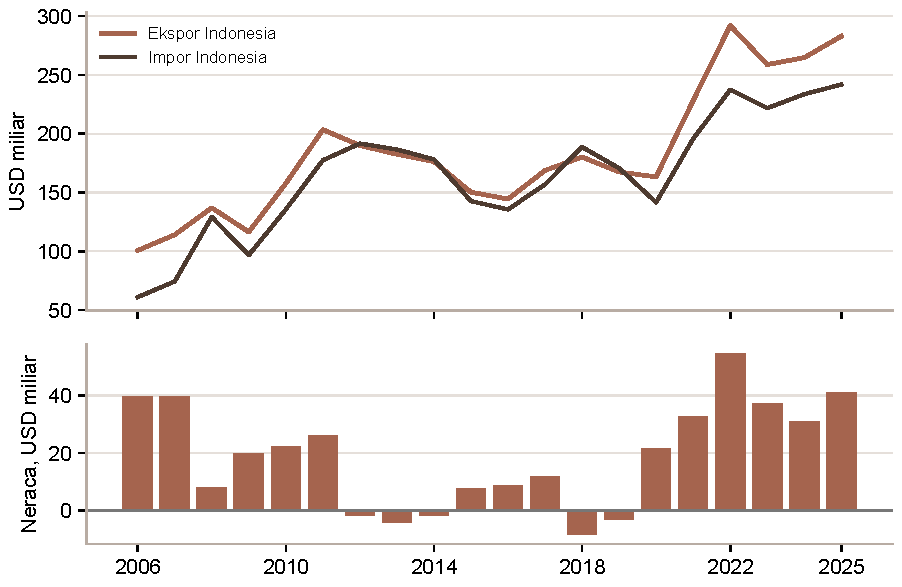
\includegraphics[width=\linewidth]{assets/indonesia_annual.pdf}
\caption{Ekspor, impor dan neraca perdagangan barang Indonesia terhadap seluruh negara. Nilai tahunan hanya menggunakan empat kuartal lengkap. Sumber: workbook Trade Map dan panel kuartalan proyek.}\label{fig:annual}
\end{figure}

\subsection{Dua dimensi klasifikasi yang bertumpang tindih}
Klasifikasi komoditas memakai kelompok A11 UNCTAD melalui korespondensi HS--SITC \cite{unctad,unsdcorr}. Komoditas total mencakup pangan, minuman, tembakau, minyak, bahan mentah pertanian, bahan bakar, serta bijih, mineral dan komoditas logam tertentu. Pertanian/pangan dan energi/tambang digunakan sebagai rinciannya. Manufaktur nonkomoditas mengikuti kategori pelengkap pada aturan tersebut, bukan identifikasi industri setiap perusahaan.

Konsumsi, modal, dan bahan baku/penolong memakai dimensi penggunaan SNA dalam BEC Rev.5 \cite{bec}. Penggunaan ini berbeda dari sifat komoditas. Produk pertanian dapat menjadi konsumsi akhir atau input antara; produk manufaktur dapat menjadi input maupun modal. Tujuh kelompok karena itu tidak merupakan partisi eksklusif. Menjumlahkan semuanya menghitung sebagian arus lebih dari sekali.

\begin{table}[!htbp]\centering\small
\caption{Kode dan definisi tujuh kelompok barang}
\begin{tabular}{p{.07\linewidth}p{.29\linewidth}p{.53\linewidth}}
\toprule Kode & Kelompok & Dasar pembentukan\\\midrule
G1 & Manufaktur nonkomoditas & Nonkomoditas UNCTAD A11 melalui SITC.\\
G2 & Barang konsumsi & BEC Rev.5, penggunaan konsumsi akhir.\\
G3 & Pertanian dan pangan & Komoditas pangan dan bahan mentah pertanian.\\
G4 & Bahan baku/penolong & BEC Rev.5, penggunaan konsumsi antara.\\
G5 & Barang modal & BEC Rev.5, pembentukan modal tetap.\\
G6 & Komoditas total & Seluruh komoditas A11 yang dapat dipetakan.\\
G7 & Energi dan tambang & Bahan bakar, bijih/mineral dan komoditas logam terkait.\\
\bottomrule\end{tabular}\label{tab:groups}
\end{table}

Workbook tidak menyatakan revisi HS untuk setiap sel. Daftar memuat kode dari beberapa revisi, sehingga kelas ditetapkan dengan konsensus konservatif per kode dari korespondensi resmi. Bila kemungkinan kelas berbeda, nilai ditandai campuran atau belum terpetakan. Nilainya tetap dalam TOTAL dan tidak dipaksakan ke kelompok tertentu. Cakupan dihitung juga per tahun, agar perubahan kode dan komposisi terlihat.

Konsensus per kode lebih rinci daripada klasifikasi HS-4, tetapi belum menjadi harmonisasi produk lintas waktu yang sempurna. Komposisi di dalam kelompok dapat berubah; hasil kelompok tidak berarti setiap kode atau perusahaan mempunyai respons sama. Kategori bahan baku/penolong menunjukkan penggunaan barang, bukan kandungan input impor eksportir.

\subsection{Kontrol makro dan keterbatasan pengukuran}
Aktivitas ekonomi menggunakan indeks level PDB riil yang ditransformasi log. Indeks pada basis rata-rata 2015 tidak boleh dijumlahkan sebagai nilai uang lintas negara. Pada bilateral digunakan GDP mitra. Pada agregat digunakan indeks sepuluh mitra dengan bobot ekspor tetap 2006--2008 dari data baru. Proksi itu merepresentasikan sebagian permintaan eksternal, tidak setara dengan GDP seluruh dunia.

Kurs agregat memakai REER BIS. Kurs bilateral dibangun dari kurs nominal dan harga, kemudian orientasinya diseragamkan agar kenaikan berarti apresiasi. Guncangan penelitian adalah perubahan kurs riil; besarnya tidak otomatis sama dengan perubahan nominal rupiah terhadap dolar. Indeks BCOM dari workbook pengguna digunakan sebagai kontrol tambahan pada sensitivitas.

India memakai CPI mulai 2013, dengan WPI sebagai pembanding terpisah. CPI Australia bulanan memuat interpolasi penyedia. Kekosongan CPI AS Oktober 2025 dan FX Vietnam Agustus 2025 dipertahankan. Beberapa GDP historis serta konsep kurs antarkompiler mempunyai catatan audit. Jejak sumber tersedia, tetapi keseragaman konsep dan vintage belum sepenuhnya terselesaikan.

\subsection{Penentuan sampel dan statistik deskriptif}
Setiap kasus memilih jendela lengkap terpanjang pada kalender kuartalan. Kuartal kosong tidak dihapus lalu dianggap berurutan. Ini menjaga arti lag, tetapi menghasilkan rentang berbeda. Baseline agregat dimulai pada data 2010Q1 demi pembandingan dengan run sebelumnya; sesudah holdback empat lag, estimasi mencakup 2011Q1--2026Q1. Perluasan 2006+ disajikan sebagai sensitivitas.

\begin{table}[!htbp]\centering
\caption{Statistik sampel estimasi agregat Indonesia, 2011Q1--2026Q1}
{\small\setlength{\tabcolsep}{3pt}\renewcommand{\arraystretch}{1.15}
\begin{tabular}{p{0.32\linewidth}p{0.045\linewidth}p{0.12\linewidth}p{0.12\linewidth}p{0.12\linewidth}p{0.12\linewidth}}
\toprule
\textbf{Variabel} & \textbf{N} & \textbf{Rerata} & \textbf{SD} & \textbf{Min.} & \textbf{Maks.}\\
\midrule
Ekspor, USD miliar & 61 & 51,15 & 12,46 & 33,60 & 78,20\\
Impor, USD miliar & 61 & 46,92 & 9,06 & 31,73 & 65,54\\
Neraca, USD miliar & 61 & 4,24 & 5,08 & -4,80 & 15,61\\
PDB riil Indonesia, indeks & 61 & 114,85 & 21,27 & 79,40 & 156,49\\
Aktivitas luar negeri, indeks & 61 & 109,43 & 13,98 & 86,16 & 135,66\\
REER, indeks & 61 & 100,99 & 4,32 & 92,89 & 111,01\\
\bottomrule
\end{tabular}
}\label{tab:desc}
\end{table}

Ekspor dan impor dalam Tabel~\ref{tab:desc} adalah nilai per kuartal. Neraca yang reratanya positif masih mempunyai kuartal defisit. Level surplus nasional karena itu tidak menjelaskan pengaruh kurs dengan sendirinya. Perdagangan belum disesuaikan musiman, sedangkan sebagian GDP memakai seri penyedia yang telah disesuaikan. Musiman masih perlu diperiksa.

\clearpage\section{Kerangka ekonomi dan metode}\label{sec:methods}
\subsection{Neraca nominal dan rasio yang diestimasi}
Untuk cakupan pasar dan barang $s$, outcome ditulis
\begin{equation}
 y_{s,t}=\ln\left(\frac{M_{s,t}}{X_{s,t}}\right),
 \qquad TB_{s,t}=X_{s,t}-M_{s,t}.\label{eq:outcome}
\end{equation}
$M$ dan $X$ adalah impor dan ekspor Indonesia. Penurunan $y$ berarti perbaikan ekspor relatif terhadap impor. Selisih dolar $TB$ digunakan sebagai statistik deskriptif, tetapi tidak di-log karena dapat negatif. Rasio menghilangkan satuan skala dolar dan mensyaratkan kedua arus positif dalam kuartal yang digunakan.

Rasio membaik tidak mengidentifikasi kenaikan ekspor secara khusus. Sebagai contoh konseptual, bila ekspor turun lima persen dan impor turun sepuluh persen, ekspor relatif terhadap impor meningkat walaupun ekspor sendiri turun. Nilai nominal juga mencampur harga dan volume. Untuk indeks harga dan volume yang konsisten secara definisi, dekomposisi konseptualnya adalah
\begin{equation}
 \ln(M/X)=\ln P_M-\ln P_X+\ln Q_M-\ln Q_X.\label{eq:value}
\end{equation}
Ini penjelasan akuntansi, bukan estimasi komponen yang tersedia dalam data. Kuantitas dan harga ekspor/impor produk belum digunakan secara langsung. BCOM adalah kontrol harga luas, bukan pengganti otomatis semua harga produk.

\subsection{J-curve dan penyesuaian perdagangan}
Harga, kontrak, dan volume dapat menyesuaikan pada waktu berbeda. Urutan J-curve memerlukan pemburukan awal setelah depresiasi, lalu perbaikan berikutnya. Kemungkinan ini tidak mengharuskan semua pasar mengikuti urutan sama. Respons yang langsung membaik merupakan hasil berbeda dari J-curve, walaupun arah akhirnya sama-sama positif.

Paper acuan mengaitkan J-curve dengan hubungan jangka pendek dan panjang dalam perdagangan bilateral \cite{bahmani}. Grafik multiplier dalam penelitian ini menggambarkan jalur penyesuaian, sementara syarat hubungan level menilai apakah hubungan akhirnya layak ditafsirkan. Kuartal ke-24 pada grafik tetap horizon simulasi terbatas. Nilai positif pada titik itu tidak otomatis membuktikan keseimbangan jangka panjang.

\subsection{ARDL sebagai pembanding linier}
Indeks $s$ selanjutnya dihilangkan agar notasi mudah dibaca. $d_t$ adalah log PDB riil Indonesia, $f_t$ log aktivitas luar negeri, dan $q_t$ kurs berorientasi apresiasi. Bentuk level ARDL adalah
\begin{equation}
 y_t=a+\sum_{\ell=1}^{p}\phi_\ell y_{t-\ell}
       +\sum_{v\in\mathcal Z}\sum_{j=0}^{q_v}b_{v,j}v_{t-j}+\varepsilon_t,
 \qquad \mathcal Z=\{d,f,q\}.\label{eq:ardl}
\end{equation}
Bila model stabil dan hubungan level didukung, koefisien jangka panjang regressor $v$ adalah
\begin{equation}
 \beta_v=\frac{\sum_{j=0}^{q_v}b_{v,j}}{1-\sum_{\ell=1}^{p}\phi_\ell}.
 \label{eq:lr}
\end{equation}
Satu koefisien kurs membatasi hubungan apresiasi dan depresiasi menjadi simetris dalam log. ARDL memberi pembanding yang lebih hemat parameter, tetapi dapat merangkum penyesuaian yang berbeda menjadi satu hubungan rata-rata. Dataset disusun dalam format panel, namun estimator yang dipakai adalah deret waktu terpisah untuk tiap kasus; bukan regresi panel yang memaksakan satu koefisien bersama.

\subsection{NARDL dan pemisahan arah kurs}
Dekomposisi partial sums adalah
\begin{align}
 q_t^+&=\sum_{j=1}^{t}\max(\Delta q_j,0),&
 q_t^-&=\sum_{j=1}^{t}\min(\Delta q_j,0),\\
 q_t&=q_0+q_t^++q_t^-.
\end{align}
Karena kenaikan $q$ berarti apresiasi, partial sum negatif mewakili depresiasi. Tanda negatifnya dipertahankan. Himpunan regressor menjadi $\mathcal Z=\{d,f,q^+,q^-\}$. Pada sensitivitas harga ditambahkan $\ln(\mathrm{BCOM})$. Ini pemisahan arah perubahan kurs, tidak sama dengan penggunaan variabel volatilitas.

Representasi error correction umumnya adalah
\begin{align}
\Delta y_t={}&\alpha+\rho y_{t-1}+\theta_d d_{t-1}+\theta_f f_{t-1}
 +\theta_+q^+_{t-1}+\theta_-q^-_{t-1}\nonumber\\
 &+\sum_{j=1}^{P}\psi_j\Delta y_{t-j}
 +\sum_{j=0}^{Q_d}\gamma_{d,j}\Delta d_{t-j}
 +\sum_{j=0}^{Q_f}\gamma_{f,j}\Delta f_{t-j}\nonumber\\
 &+\sum_{j=0}^{Q_+}\pi_j^+\Delta q^+_{t-j}
 +\sum_{j=0}^{Q_-}\pi_j^-\Delta q^-_{t-j}+\eta_t.
 \label{eq:ecm}
\end{align}
Koefisien dapat nol atau terikat sesuai lag level yang terpilih. Bentuk ini menjelaskan struktur umum, bukan klaim bahwa semua suku diestimasi bebas pada setiap kasus. Normalisasi memenuhi
\begin{equation}
 \rho=\sum_{\ell=1}^{p}\phi_\ell-1,\qquad
 \beta_-=-\theta_-/\rho,\qquad \beta_+=-\theta_+/\rho.
\end{equation}
Tanda $\rho<0$ konsisten dengan koreksi deviasi, tetapi belum cukup sendirian untuk mengesahkan hubungan level.

\subsection{Orientasi kurs dan tanda koefisien}
Agregat menggunakan $q_t=\ln(\mathrm{REER}_t)$. Bilateral menggunakan negatif log RER panel agar kenaikan juga berarti apresiasi. Untuk depresiasi $\delta^-<0$, perubahan jangka panjang yang diimplikasikan koefisien adalah
\begin{equation}
 \Delta y_\infty^-=\beta_-\delta^-.
\end{equation}
Karena $y$ adalah log impor/ekspor, $\beta_->0$ mengarah pada perbaikan ketika dikalikan guncangan negatif. Koefisien negatif mengarah pada pemburukan. Definisi ini harus diperiksa terlebih dahulu bila pembaca terbiasa dengan ekspor/impor sebagai outcome.

Grafik paper dan PPT memakai transformasi tepat
\begin{equation}
 R_h^J=-100\,\Delta_h y=100\,\Delta_h\ln(X/M).\label{eq:display}
\end{equation}
Positif berarti perbaikan, dengan interval ikut dibalik dan batasnya ditukar. Guncangannya adalah $\delta^-=-\ln(1.10)$ serta $\delta^+=+\ln(1.10)$. Keduanya simetris dalam log. Dalam persen aritmetika, kenaikan indeks sepuluh persen berpasangan dengan penurunan sekitar 9,09 persen, bukan dua perubahan sepuluh persen yang sama besar.

\subsection{Proksi aktivitas luar negeri}
Bilateral memakai GDP mitra. Proksi agregat dibentuk sebagai
\begin{equation}
 f_t=\ln\left(\sum_{i=1}^{10}w_iY^{(2015=100)}_{i,t}\right),
 \qquad \sum_{i=1}^{10}w_i=1.
\end{equation}
Bobot $w_i$ adalah pangsa ekspor tetap 2006--2008 di antara sepuluh mitra. Penggunaan indeks menghindari penjumlahan GDP dalam mata uang yang berbeda, tetapi tetap membatasi representasi permintaan asing. Bobot tidak mengikuti perubahan komposisi ekspor, dan negara di luar sepuluh mitra tidak terwakili langsung. Proksi ini bukan GDP seluruh dunia.

\subsection{Lag dan sampel efektif}
AIC memilih lag level dengan maksimum empat. Maksimum dua dijalankan sebagai sensitivitas. Kriteria yang digunakan sepadan dengan
\begin{equation}
 \mathrm{AIC}=N\ln(\mathrm{RSS}/N)+2K,\qquad
 \mathrm{BIC}=N\ln(\mathrm{RSS}/N)+K\ln N,
\end{equation}
dengan $K$ jumlah parameter. Dalam suatu cap, ARDL dan NARDL memakai holdback maksimum yang sama. Cap dua dapat memasukkan dua kuartal lebih awal daripada cap empat. Perbandingannya karena itu mengubah batas lag sekaligus sedikit mengubah window, belum menjadi uji panjang lag pada sampel yang persis sama.

Paper pengguna memilih maksimum delapan lag first difference pada sampel jauh lebih panjang. Empat lag level di sini adalah adaptasi terhadap keterbatasan sampel, bukan padanan mekanis delapan lag first difference. Banyaknya parameter, terutama pada NARDL dengan tambahan BCOM, perlu dibaca bersama jumlah kuartal dan derajat bebas residual.

\subsection{Unit root dan penyaringan hubungan level}
Bounds memakai F dan t serta probabilitas finite-sample implementasi \texttt{ardl} \cite{pss,ks}. Keputusan utama lima persen mensyaratkan penolakan menurut keduanya. Penyaringan level tambahan memerlukan penolakan joint-X, akar dinamis stabil, tidak ada flag risiko integrasi orde dua, dan minimal 15 derajat bebas residual. Joint-X membantu memastikan penolakan melibatkan regressor level dan tidak hanya dinamika outcome.

ADF memilih lag melalui BIC pada kandidat nol sampai empat; PP memakai empat lag. ADF dengan tren juga dilaporkan pada level. Flag integrasi orde dua dibuat ketika ADF dan PP pada first difference sama-sama gagal menolak pada sepuluh persen untuk variabel yang digunakan. Ini peringatan operasional, bukan diagnosis pasti bahwa variabel berorde dua. Kegagalan menolak dapat mencerminkan daya uji rendah. Dukungan level yang dilaporkan harus dipahami dengan syarat-syarat tersebut.

Paper acuan juga membahas sejumlah hasil pada taraf sepuluh persen. Run ini menyimpan keputusan F-only sepuluh persen sebagai pembanding bergaya paper, tetapi kesimpulan utama memakai F dan t lima persen serta penyaringan tambahan. Karena ambang dan kriterianya berbeda, jumlah model yang dinilai mendukung tidak boleh diklaim mereplikasi keputusan paper secara identik. Pemilihan ambang tidak diubah setelah melihat tanda hasil.

\subsection{Asimetri, multiplier, dan interval}
Asimetri jangka panjang diuji melalui $H_0:\beta_+=\beta_-$. Pembandingan jangka pendek memakai jumlah koefisien perubahan partial sums dalam parameterisasi yang digunakan. Penolakan Wald dan keberadaan hubungan level menjawab pertanyaan berbeda. Asimetri pada model yang belum mendukung level belum cukup untuk menyatakan perbedaan jangka panjang yang mapan.

Multiplier dan respons tampilan memenuhi
\begin{equation}
 m_h^\pm=\frac{\partial y_{t+h}}{\partial q_t^\pm},\qquad
 R_h^{J,\pm}=-100\,m_h^\pm\delta^\pm,\qquad h=0,\ldots,24.
\end{equation}
Band nominal 95\% dihitung melalui delta method dari kovarians persamaan level dan kuantil t residual. Band bersifat pointwise, tidak simultan seluruh jalur. Pemilihan AIC terjadi sebelum inferensi, sehingga interval belum mengoreksi ketidakpastian seleksi lag.

Koreksi Benjamini--Hochberg (BH) \cite{bh} digunakan secara eksploratif dalam keluarga cakupan dan estimator model utama. Keluarga agregat berisi satu model per estimator, bilateral sepuluh, dan barang 77. Koreksi ini bukan pengendalian lengkap pencarian 516 model, terutama karena kelompok bertumpang tindih dan sensitivitas juga diperiksa.

\readingbox{\textbf{Urutan pembacaan.} Periksa outcome dan orientasi kurs, kemudian dukungan level, besarnya koefisien serta interval, diagnostik, dan sensitivitas. Probabilitas koefisien yang kecil tidak menggantikan pemeriksaan lainnya.}

\clearpage\section{Hasil agregat perdagangan Indonesia}\label{sec:aggregate}
\subsection{Dukungan level belum kuat pada model utama}
Agregat menggabungkan ekspor dan impor Indonesia dengan seluruh negara. Kedua model utama menggunakan 61 kuartal pada 2011Q1--2026Q1. ARDL memilih lag level $(2,3,0,4)$ untuk outcome, GDP Indonesia, aktivitas luar negeri dan kurs. NARDL memilih $(2,0,3,0,4)$, dengan dua posisi terakhir untuk partial sums positif dan negatif. Perbedaan lag ini merupakan hasil AIC pada himpunan kandidat, bukan bukti bahwa lag tersebut pasti menggambarkan proses ekonomi sebenarnya.

\begin{table}[!htbp]\centering
\caption{Bounds dan joint-X untuk agregat Indonesia}
{\small\setlength{\tabcolsep}{3pt}\renewcommand{\arraystretch}{1.15}
\begin{tabular}{p{0.1\linewidth}p{0.08\linewidth}p{0.08\linewidth}p{0.1\linewidth}p{0.1\linewidth}p{0.12\linewidth}p{0.22\linewidth}}
\toprule
\textbf{Model} & \textbf{F} & \textbf{t} & \textbf{p F(I1)} & \textbf{p t(I1)} & \textbf{p joint-X} & \textbf{Keputusan}\\
\midrule
ARDL & 2,481 & -2,280 & 0,369 & 0,434 & 0,259 & No rejection\\
NARDL & 3,799 & -2,887 & 0,094 & 0,279 & 0,011 & Inconclusive\\
\bottomrule
\end{tabular}
}\label{tab:worldbounds}
\end{table}

ARDL menghasilkan koefisien kurs sekitar 0,429 dengan probabilitas nominal 0,661. Intervalnya melintasi nol dan F/t bounds belum menolak tidak adanya hubungan level. Diagnostik residual yang tidak ditolak pada model ini tidak mengubah hasil bounds menjadi dukungan jangka panjang. Kasus ini memperlihatkan bahwa diagnostik dan keberadaan hubungan level merupakan dua pemeriksaan yang terpisah.

Pada NARDL, koefisien depresiasi sekitar 2,572 dengan probabilitas nominal 0,040. Koefisien apresiasi sekitar $-2,142$, sedangkan probabilitas Wald kesamaan keduanya sekitar 0,006. Bila hanya koefisien dan bintang yang dibaca, hasilnya tampak mendukung hubungan yang asimetris dan menguntungkan saat depresiasi. Namun probabilitas upper-bound F sekitar 0,094 dan t sekitar 0,279, sehingga keputusan bersama lima persen belum terpenuhi. Catatan CUSUMSQ juga membatasi pembacaan stabilitas.

\begin{figure}[!htbp]\centering
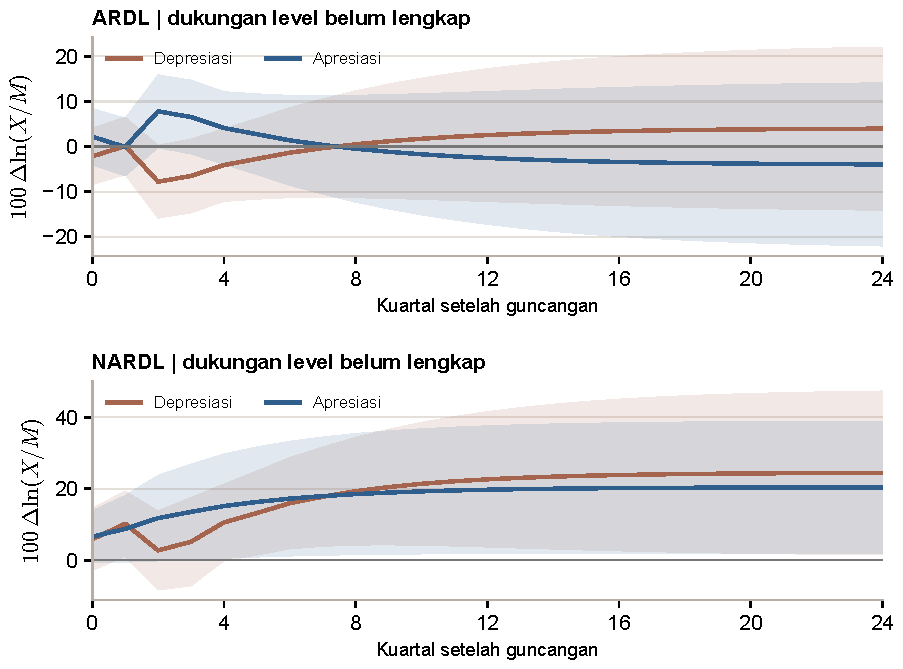
\includegraphics[width=\linewidth]{assets/response_WORLD.pdf}
\caption{Respons agregat perdagangan Indonesia. Cokelat menunjukkan depresiasi dan biru apresiasi; area berwarna adalah CI pointwise nominal 95\%. Positif berarti rasio ekspor/impor membaik. Skala vertikal dua panel berbeda.}\label{fig:world}
\end{figure}

\subsection{Apa yang dapat dipelajari dari bentuk respons}
ARDL memperlihatkan pemburukan awal pada estimasi titik sebelum perbaikan pada horizon berikutnya. Band cukup lebar, termasuk di sekitar nol pada bagian penting jalur. NARDL lebih banyak mengarah pada perbaikan, dengan fluktuasi awal yang belum menghasilkan bukti pemburukan terukur. Perbandingan ini memberi informasi mengenai bentuk yang diimplikasikan spesifikasi, tetapi tidak menggantikan syarat level yang belum terpenuhi.

Kedua arah kurs pada NARDL dapat sama-sama tampak memperbaiki rasio. Hal itu berasal dari koefisien dua partial sums yang berbeda tanda pada outcome impor/ekspor. Hasil tersebut tidak boleh langsung diperlakukan sebagai pilihan kebijakan bahwa kedua arah perubahan kurs sama-sama memberikan manfaat. Partial sums merangkum jalur historis yang berbeda, berhubungan dengan regressor lain, dan diestimasi pada sampel terbatas. Penggunaan bahasa hubungan kondisional menjadi penting ketika hasilnya tidak mendukung struktur keseimbangan yang kuat.

Baseline agregat 2010+ dipertahankan untuk pembandingan dengan run sebelumnya; perdagangan baru sendiri berasal dari workbook HS-6 pengguna. Perluasan data menjadi 2006+ tetap diestimasi dan dilaporkan dalam sensitivitas. Memilih salah satu window karena koefisiennya lebih sesuai harapan akan memperbesar risiko pencarian hasil. Kesimpulan agregat yang dapat dipertahankan adalah bahwa model utama belum memberikan hubungan jangka panjang yang kuat, bukan bahwa depresiasi terbukti tidak mempunyai pengaruh apa pun.

\subsection{Membaca arti angka tanpa mengubahnya menjadi ramalan}
Contoh yang lebih mendukung tersedia pada NARDL Indonesia--Australia. Dengan koefisien $\widehat{\beta}_-=\AusBetaMath$ dan guncangan log $-\ln(1.10)$, perubahan tampilan jangka panjang yang diimplikasikan adalah
\begin{equation}
 -100\,\widehat{\beta}_-\big[-\ln(1.10)\big]
 \simeq \AusResponseMath.
\end{equation}
Angka \AusResponse{} adalah poin log kali seratus. Perubahan persentase rasio ekspor/impor yang bersesuaian, secara aljabar, adalah
\begin{equation}
 100\left[\exp\{-\widehat{\beta}_-\delta^-\}-1\right].
\end{equation}
Pada titik estimasi itu hasilnya sekitar \AusRatioPct\%. Angka tersebut bukan peningkatan surplus dolar sebesar \AusRatioPct\%, bukan kenaikan ekspor dengan persentase yang sama, dan bukan prakiraan kebijakan tanpa syarat. Contoh ini hanya menerjemahkan satu koefisien model ke skala rasio, sambil mempertahankan seluruh asumsi dan ketidakpastian model asalnya.

\clearpage\section{Hasil bilateral sepuluh mitra}\label{sec:bilateral}

\subsection{Perbedaan arah dan dukungan model}

Hasil bilateral membedakan satu hubungan agregat menjadi sepuluh pengalaman pasar. Tabel berikut memakai koefisien depresiasi NARDL dan window setelah holdback. Australia dan Malaysia memenuhi penyaringan level serta diagnostik utama, tetapi signifikansi keduanya tidak sama tahan terhadap BH. Model lain tetap dilaporkan walaupun mempunyai koefisien besar atau probabilitas kecil tanpa dukungan level lengkap.

\begin{table}[!htbp]\centering\caption{Ringkasan NARDL bilateral Indonesia}{\small\setlength{\tabcolsep}{3pt}\renewcommand{\arraystretch}{1.15}
\begin{tabular}{p{0.17\linewidth}p{0.045\linewidth}p{0.2\linewidth}p{0.12\linewidth}p{0.09\linewidth}p{0.09\linewidth}p{0.07\linewidth}}
\toprule
\textbf{Mitra} & \textbf{N} & \textbf{Rentang} & \textbf{Koef. dep.} & \textbf{p} & \textbf{BH} & \textbf{Status}\\
\midrule
Australia & 77 & 2007Q1--2026Q1 & 3,356 & \(<0{,}001\) & 0,004 & L+D\\
Tiongkok & 78 & 2007Q1--2026Q2 & -2,727 & 0,250 & 0,350 & --\\
India & 49 & 2014Q1--2026Q1 & -6,443 & 0,236 & 0,350 & --\\
Jepang & 78 & 2007Q1--2026Q2 & -2,456 & 0,006 & 0,020 & --\\
Korea Selatan & 78 & 2007Q1--2026Q2 & 3,935 & 0,144 & 0,288 & --\\
Malaysia & 78 & 2007Q1--2026Q2 & 1,346 & 0,024 & 0,059 & L+D\\
Singapura & 78 & 2007Q1--2026Q2 & -0,262 & 0,810 & 0,810 & --\\
Thailand & 78 & 2007Q1--2026Q2 & 0,950 & 0,280 & 0,350 & L\\
Amerika Serikat & 75 & 2007Q1--2025Q3 & 3,095 & 0,006 & 0,020 & --\\
Vietnam & 74 & 2007Q1--2025Q2 & -0,551 & 0,737 & 0,810 & --\\
\bottomrule
\end{tabular}
}\label{tab:bilateral}\end{table}

\begin{figure}[!htbp]\centering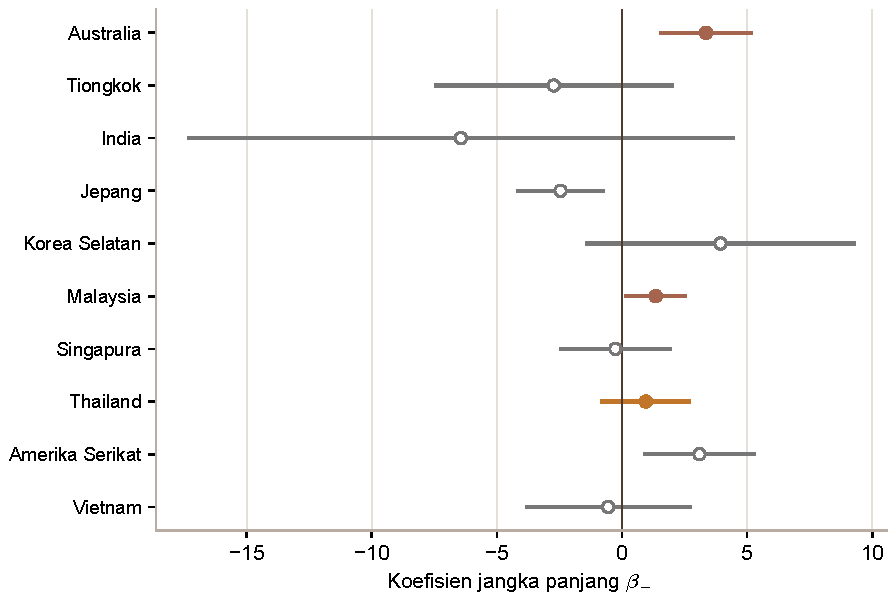
\includegraphics[width=\linewidth]{assets/bilateral_forest.pdf}\caption{Koefisien depresiasi bilateral NARDL. Warna cokelat menunjukkan L+D, emas L, dan simbol kosong dukungan level belum lengkap. Semua negara pada sumbu adalah mitra Indonesia.}\label{fig:bilateralforest}\end{figure}


Perbedaan antarmitra belum merupakan uji formal selisih koefisien pada sampel sama. India berawal lebih akhir, sedangkan AS dan Vietnam berakhir lebih awal. Regresi yang berbeda juga mengendalikan GDP dan kurs bilateral yang berbeda. Uraian tiap mitra berikut menghubungkan angka, status dan grafik agar penafsiran tidak bergantung pada satu kolom bintang.

\clearpage\subsection{Indonesia--Australia}

NARDL Indonesia--Australia memakai 77 kuartal pada 2007Q1--2026Q1. Koefisien depresiasi 3,356, CI nominal 95\% [1,563; 5,149], probabilitas nominal \(<0{,}001\), dan BH 0,004. Probabilitas asimetri jangka panjang 0,147. Pemeriksaan yang membatasi: tidak ada penolakan pada penyaringan yang digunakan.

Australia menjadi contoh yang lebih mendukung perbaikan rasio neraca saat depresiasi. ARDL dan NARDL sama-sama memenuhi penyaringan level dan diagnostik. Koefisien depresiasi NARDL tetap signifikan setelah BH dalam keluarga bilateral, sedangkan Wald kesamaan apresiasi dan depresiasi tidak ditolak pada lima persen. Pemakaian NARDL karena itu tidak berarti asimetri pasti ditemukan.

Estimasi titik NARDL mempunyai pemburukan awal lalu perbaikan. Band awal masih melintasi nol, sehingga urutan J tidak terkonfirmasi sama kuat pada dua fase. Pernyataan yang lebih tepat adalah adanya pola J pada titik yang didukung kelayakan model, dengan ketidakpastian fase awal. Ini berbeda dari menyatakan depresiasi pasti menurunkan neraca pada kuartal pertama.

\begin{figure}[!htbp]\centering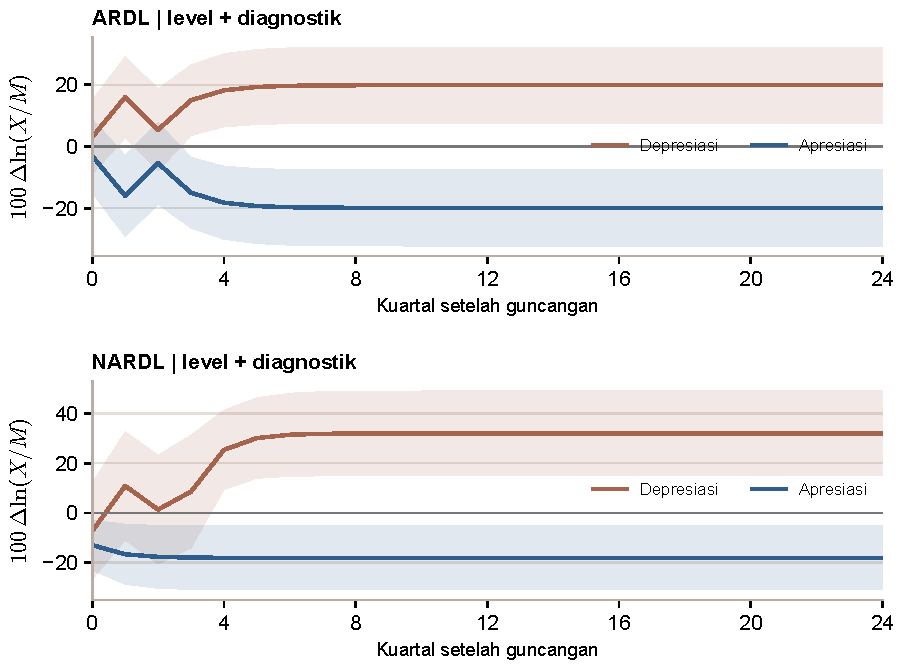
\includegraphics[width=\linewidth]{assets/response_BIL_AUS.pdf}\caption{Respons perdagangan Indonesia--Australia. Positif berarti perbaikan rasio ekspor/impor. Band pointwise nominal 95\%; skala kedua panel berbeda.}\label{fig:bilAUS}\end{figure}


\clearpage\subsection{Indonesia--Tiongkok}

NARDL Indonesia--Tiongkok memakai 78 kuartal pada 2007Q1--2026Q2. Koefisien depresiasi -2,727, CI nominal 95\% [-7,427; 1,972], probabilitas nominal 0,250, dan BH 0,350. Probabilitas asimetri jangka panjang 0,905. Pemeriksaan yang membatasi: F/t bounds belum menolak; joint-X belum menolak; catatan diagnostik residual/stabilitas.

Besarnya nilai perdagangan dengan Tiongkok tidak membuat koefisiennya otomatis paling presisi atau paling dapat ditafsirkan. Kedua model bilateral utama belum memenuhi syarat level lengkap. Pada NARDL terdapat catatan korelasi serial; pada ARDL CUSUM ditolak. Arah negatif belum dapat dipakai sebagai bukti jangka panjang bahwa depresiasi merugikan seluruh perdagangan Indonesia dengan Tiongkok.

Hasil kelompok pertanian dengan Tiongkok kemudian memberi gambaran yang lebih terukur. Perbedaan hasil total dan kelompok menandai peran agregasi, tetapi belum merupakan uji bahwa kedua koefisiennya berbeda secara statistik. Defisit bilateral yang besar pada statistik tahunan juga tidak mengidentifikasi sebab akibat dari perubahan kurs.

\begin{figure}[!htbp]\centering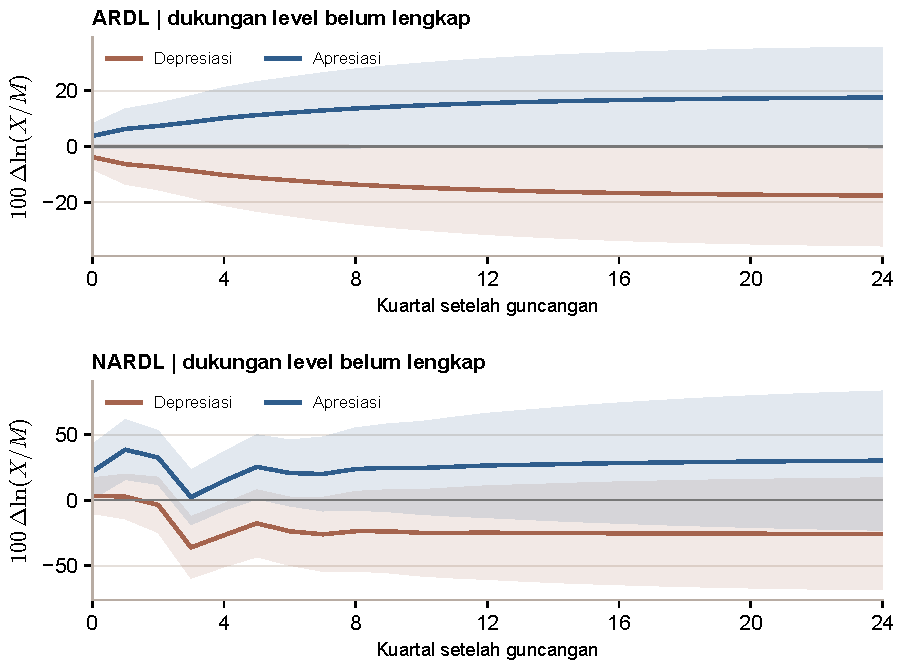
\includegraphics[width=\linewidth]{assets/response_BIL_CHN.pdf}\caption{Respons perdagangan Indonesia--Tiongkok. Positif berarti perbaikan rasio ekspor/impor. Band pointwise nominal 95\%; skala kedua panel berbeda.}\label{fig:bilCHN}\end{figure}


\clearpage\subsection{Indonesia--India}

NARDL Indonesia--India memakai 49 kuartal pada 2014Q1--2026Q1. Koefisien depresiasi -6,443, CI nominal 95\% [-17,300; 4,414], probabilitas nominal 0,236, dan BH 0,350. Probabilitas asimetri jangka panjang 0,021. Pemeriksaan yang membatasi: F/t bounds belum menolak; joint-X belum menolak.

India memakai sampel yang lebih pendek karena baseline menggunakan CPI mulai 2013. Dengan tambahan partial sums dan lag, ruang informasi per parameter menjadi terbatas. Koefisien depresiasi NARDL negatif tetapi intervalnya lebar; bounds belum mendukung level. Penolakan Wald asimetri tidak mengatasi masalah tersebut.

Model NARDL tidak ditolak pada penyaringan residual yang dipakai, sedangkan ARDL mempunyai catatan korelasi serial dan RESET. Ini contoh model yang residualnya tampak lebih mendukung tetapi hubungan levelnya belum memenuhi syarat. WPI menyediakan sensitivitas terpisah dengan konsep harga serta rentang yang berbeda; ia tidak diperlakukan sebagai CPI murni untuk memperpanjang baseline.

\begin{figure}[!htbp]\centering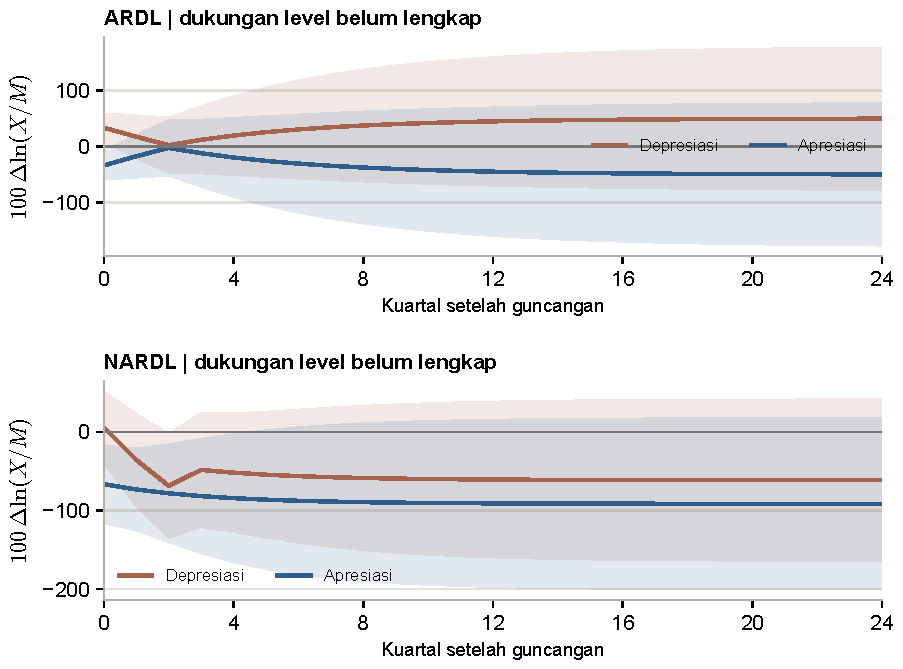
\includegraphics[width=\linewidth]{assets/response_BIL_IND.pdf}\caption{Respons perdagangan Indonesia--India. Positif berarti perbaikan rasio ekspor/impor. Band pointwise nominal 95\%; skala kedua panel berbeda.}\label{fig:bilIND}\end{figure}


\clearpage\subsection{Indonesia--Jepang}

NARDL Indonesia--Jepang memakai 78 kuartal pada 2007Q1--2026Q2. Koefisien depresiasi -2,456, CI nominal 95\% [-4,166; -0,747], probabilitas nominal 0,006, dan BH 0,020. Probabilitas asimetri jangka panjang 0,971. Pemeriksaan yang membatasi: F/t bounds belum menolak; catatan diagnostik residual/stabilitas.

Jepang memperlihatkan mengapa probabilitas koefisien saja dapat menyesatkan. Koefisien depresiasi NARDL negatif dan signifikan nominal maupun BH dalam keluarga bilateral. F upper bound menolak pada lima persen, tetapi t upper bound belum melewati ambang yang sama. Penyaringan hubungan level lengkap karena itu belum terpenuhi.

Selain itu, ARCH dan normalitas residual memberi catatan. Hasil ini tidak dihapus dari pelaporan, tetapi bobot penafsirannya berbeda dari kasus yang mendukung level dan diagnostik. Tanda negatif menjadi indikasi yang memerlukan peninjauan spesifikasi, bukan kesimpulan kausal mengenai respons ekspor Indonesia ke Jepang.

\begin{figure}[!htbp]\centering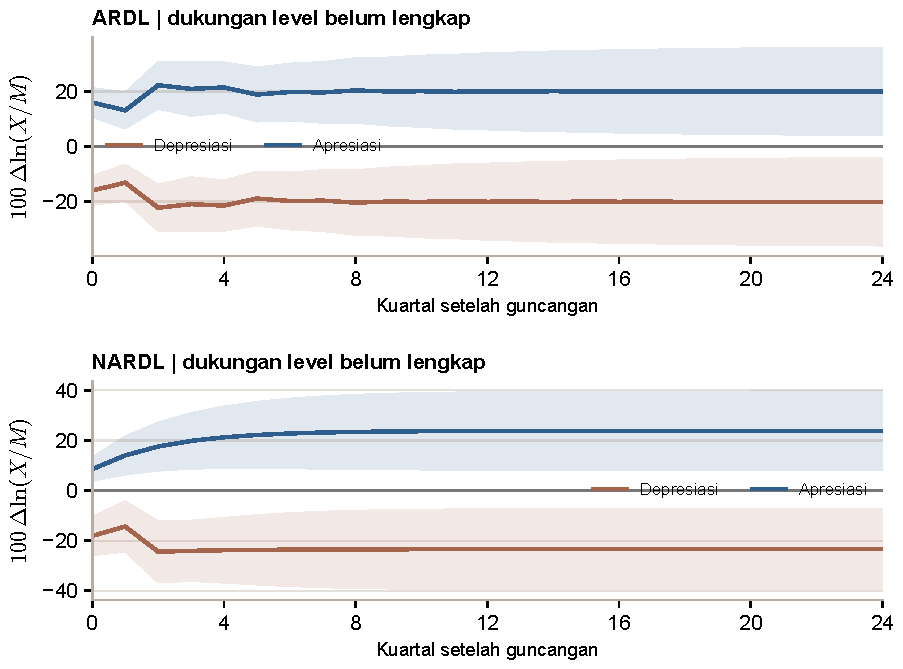
\includegraphics[width=\linewidth]{assets/response_BIL_JPN.pdf}\caption{Respons perdagangan Indonesia--Jepang. Positif berarti perbaikan rasio ekspor/impor. Band pointwise nominal 95\%; skala kedua panel berbeda.}\label{fig:bilJPN}\end{figure}


\clearpage\subsection{Indonesia--Korea Selatan}

NARDL Indonesia--Korea Selatan memakai 78 kuartal pada 2007Q1--2026Q2. Koefisien depresiasi 3,935, CI nominal 95\% [-1,383; 9,253], probabilitas nominal 0,144, dan BH 0,288. Probabilitas asimetri jangka panjang 0,112. Pemeriksaan yang membatasi: F/t bounds belum menolak; joint-X belum menolak; catatan diagnostik residual/stabilitas.

NARDL Korea menghasilkan koefisien depresiasi positif dengan ketidakpastian yang cukup besar. Dukungan level belum lengkap, dan korelasi serial, RESET serta CUSUM memberi catatan. ARDL lebih dekat ke nol tetapi juga belum mendukung level. Kedua hasil belum menetapkan bahwa efek nasional pada mitra ini kecil ataupun positif secara pasti.

Pada kelompok modal, NARDL mempunyai pola J yang lebih jelas dan lolos penyaringan utama. Kontras ini menunjukkan bahwa hasil agregat mitra dapat menyembunyikan respons kelompok tertentu. Kelompok modal tetap tidak mewakili semua ekspor ke Korea, dan band jalurnya masih bersifat pointwise.

\begin{figure}[!htbp]\centering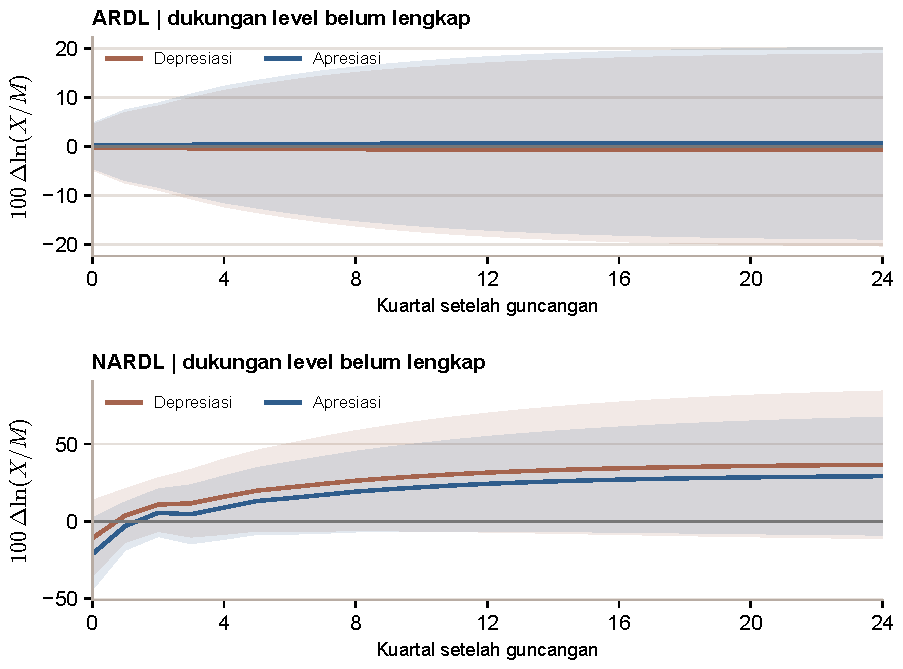
\includegraphics[width=\linewidth]{assets/response_BIL_KOR.pdf}\caption{Respons perdagangan Indonesia--Korea Selatan. Positif berarti perbaikan rasio ekspor/impor. Band pointwise nominal 95\%; skala kedua panel berbeda.}\label{fig:bilKOR}\end{figure}


\clearpage\subsection{Indonesia--Malaysia}

NARDL Indonesia--Malaysia memakai 78 kuartal pada 2007Q1--2026Q2. Koefisien depresiasi 1,346, CI nominal 95\% [0,186; 2,507], probabilitas nominal 0,024, dan BH 0,059. Probabilitas asimetri jangka panjang \(<0{,}001\). Pemeriksaan yang membatasi: tidak ada penolakan pada penyaringan yang digunakan.

Malaysia menunjukkan perbedaan yang nyata antara spesifikasi linier dan nonlinear. ARDL mempunyai dukungan level tetapi koefisien kursnya negatif, tidak signifikan pada lima persen, serta mempunyai catatan RESET dan CUSUM. NARDL memberi koefisien depresiasi positif, dukungan level dan diagnostik yang lebih baik, serta penolakan asimetri.

Probabilitas depresiasi NARDL sekitar 0,024 secara nominal, tetapi BH sekitar 0,059. Dengan demikian, klaim signifikansinya berubah menurut apakah pengujian berganda diperhitungkan. Respons yang cenderung membaik tidak harus diberi nama J-curve apabila fase awal yang memburuk tidak muncul. Temuan ini mendukung pembacaan perbaikan kondisional dengan ketahanan signifikansi yang terbatas.

\begin{figure}[!htbp]\centering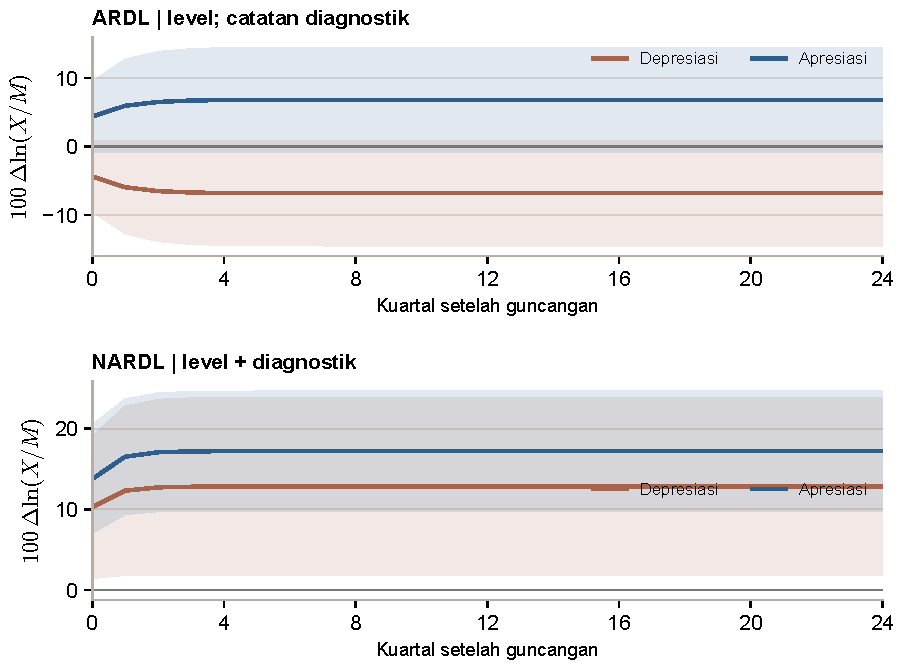
\includegraphics[width=\linewidth]{assets/response_BIL_MYS.pdf}\caption{Respons perdagangan Indonesia--Malaysia. Positif berarti perbaikan rasio ekspor/impor. Band pointwise nominal 95\%; skala kedua panel berbeda.}\label{fig:bilMYS}\end{figure}


\clearpage\subsection{Indonesia--Singapura}

NARDL Indonesia--Singapura memakai 78 kuartal pada 2007Q1--2026Q2. Koefisien depresiasi -0,262, CI nominal 95\% [-2,440; 1,915], probabilitas nominal 0,810, dan BH 0,810. Probabilitas asimetri jangka panjang 0,791. Pemeriksaan yang membatasi: joint-X belum menolak; catatan diagnostik residual/stabilitas.

Pada Singapura, F dan t bounds dapat menolak sementara joint-X tidak mendukung. Keputusan level lengkap karena itu tetap belum lolos. ARDL juga memberi contoh bahwa diagnostik yang tidak ditolak tidak cukup bila komponen level regressor belum terdukung. NARDL menambahkan catatan korelasi serial.

Koefisien depresiasi NARDL dekat nol dalam titik dibandingkan beberapa mitra lain, tetapi intervalnya tetap harus dibaca sebelum menyebut ketidakpekaan. Run ini tidak melakukan uji ekuivalensi efek kecil. Hasil yang paling dapat dipertahankan adalah belum adanya hubungan jangka panjang yang cukup didukung pada spesifikasi utama.

\begin{figure}[!htbp]\centering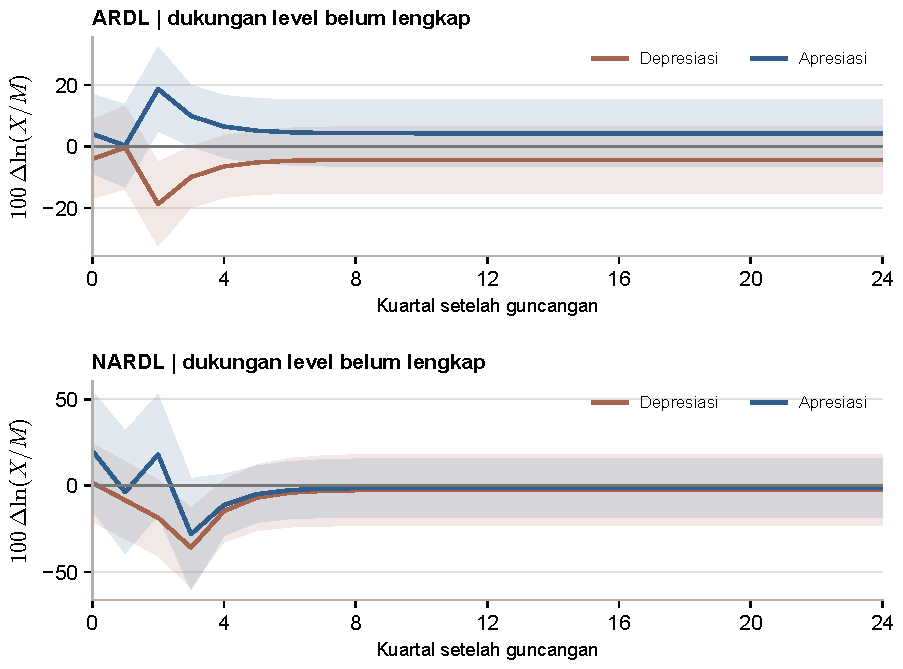
\includegraphics[width=\linewidth]{assets/response_BIL_SGP.pdf}\caption{Respons perdagangan Indonesia--Singapura. Positif berarti perbaikan rasio ekspor/impor. Band pointwise nominal 95\%; skala kedua panel berbeda.}\label{fig:bilSGP}\end{figure}


\clearpage\subsection{Indonesia--Thailand}

NARDL Indonesia--Thailand memakai 78 kuartal pada 2007Q1--2026Q2. Koefisien depresiasi 0,950, CI nominal 95\% [-0,789; 2,690], probabilitas nominal 0,280, dan BH 0,350. Probabilitas asimetri jangka panjang 0,765. Pemeriksaan yang membatasi: catatan diagnostik residual/stabilitas.

Thailand berbeda dari banyak pasangan karena kedua model memenuhi syarat level operasional. Namun ARCH dan CUSUMSQ ditolak, dengan tambahan CUSUM pada NARDL. Dukungan kointegrasi dan kestabilan residual karena itu tidak bergerak bersama. Koefisien positif NARDL juga belum signifikan secara nominal.

Kurs Thailand mempunyai catatan perbedaan konsep antarcompiler. Keluarga GEM dijalankan penuh sebagai sensitivitas, bukan digunakan untuk menambal satu observasi baseline. Perbandingan sumber tetap perlu memperhatikan apakah window dan definisinya sama. Sampai isu tersebut diperiksa lebih jauh, koefisien tidak dibaca sebagai efek kebijakan yang telah stabil.

\begin{figure}[!htbp]\centering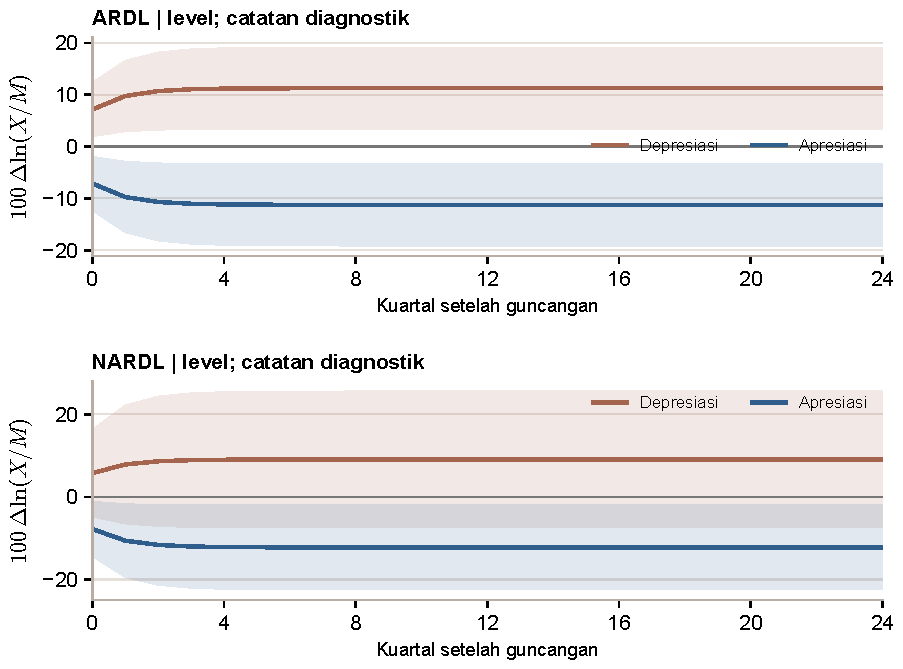
\includegraphics[width=\linewidth]{assets/response_BIL_THA.pdf}\caption{Respons perdagangan Indonesia--Thailand. Positif berarti perbaikan rasio ekspor/impor. Band pointwise nominal 95\%; skala kedua panel berbeda.}\label{fig:bilTHA}\end{figure}


\clearpage\subsection{Indonesia--Amerika Serikat}

NARDL Indonesia--Amerika Serikat memakai 75 kuartal pada 2007Q1--2025Q3. Koefisien depresiasi 3,095, CI nominal 95\% [0,921; 5,269], probabilitas nominal 0,006, dan BH 0,020. Probabilitas asimetri jangka panjang 0,240. Pemeriksaan yang membatasi: joint-X belum menolak; catatan diagnostik residual/stabilitas.

AS menghasilkan koefisien depresiasi NARDL yang positif dan signifikan nominal maupun BH. F dan t bounds juga menolak. Namun joint-X sekitar 0,060 belum melewati ambang lima persen, sehingga syarat level tambahan tidak terpenuhi. CUSUMSQ dan normalitas residual memberi catatan lain.

Sampel berhenti pada 2025Q3 akibat kekosongan CPI Oktober 2025 pada keluarga utama. Kelompok konsumsi dengan AS mempunyai dukungan berbeda dan memperlihatkan pola J yang lebih jelas. Hal tersebut tidak menyelesaikan kekurangan model total, karena agregasi barang dan persamaan yang diuji berbeda.

\begin{figure}[!htbp]\centering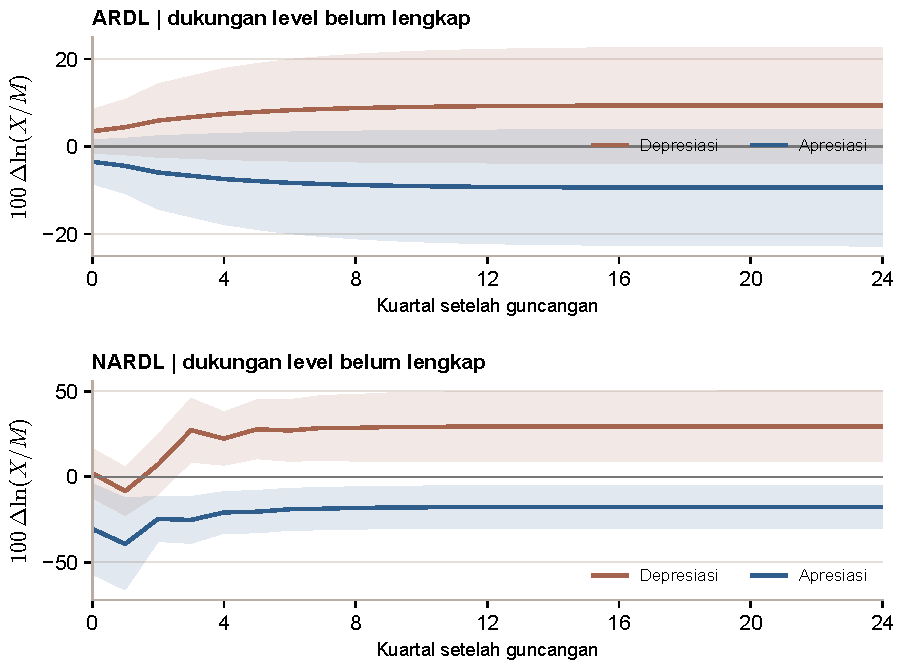
\includegraphics[width=\linewidth]{assets/response_BIL_USA.pdf}\caption{Respons perdagangan Indonesia--Amerika Serikat. Positif berarti perbaikan rasio ekspor/impor. Band pointwise nominal 95\%; skala kedua panel berbeda.}\label{fig:bilUSA}\end{figure}


\clearpage\subsection{Indonesia--Vietnam}

NARDL Indonesia--Vietnam memakai 74 kuartal pada 2007Q1--2025Q2. Koefisien depresiasi -0,551, CI nominal 95\% [-3,806; 2,704], probabilitas nominal 0,737, dan BH 0,810. Probabilitas asimetri jangka panjang 0,163. Pemeriksaan yang membatasi: F/t bounds belum menolak; catatan diagnostik residual/stabilitas.

Vietnam mempunyai catatan varians dan stabilitas yang cukup luas. NARDL memberikan koefisien depresiasi negatif yang tidak signifikan, sedangkan t bounds belum mendukung keputusan level. ARDL juga belum memenuhi seluruh syarat dan menolak beberapa diagnostik. Koefisien tidak dipilih hanya karena arahnya sesuai atau bertentangan dengan hipotesis.

Kekosongan kurs Agustus 2025 memotong jendela utama yang lengkap pada 2025Q2. Prosedur tidak merapatkan kuartal setelah celah dan menganggapnya berurutan. Alternatif GEM tetap merupakan sensitivitas dengan konsep sumber yang mungkin berbeda. Keterbatasan itu memengaruhi perbandingan Vietnam dengan mitra yang berakhir lebih akhir.

\begin{figure}[!htbp]\centering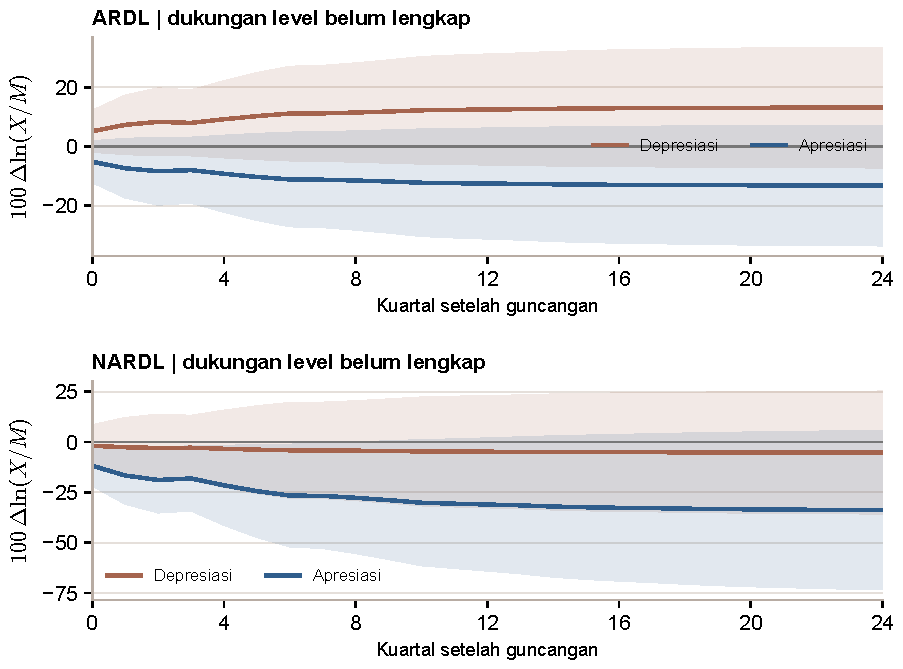
\includegraphics[width=\linewidth]{assets/response_BIL_VNM.pdf}\caption{Respons perdagangan Indonesia--Vietnam. Positif berarti perbaikan rasio ekspor/impor. Band pointwise nominal 95\%; skala kedua panel berbeda.}\label{fig:bilVNM}\end{figure}

\clearpage\section{Hasil menurut kelompok barang HS-6}\label{sec:goods}
\subsection{Gambaran agregat Indonesia menurut tujuh kelompok}
Disaggregasi barang memperlihatkan informasi yang tidak sama dengan hasil total. Tabel~\ref{tab:goodslr} melaporkan koefisien yang relevan untuk depresiasi: koefisien kurs pada ARDL dan koefisien partial sum negatif pada NARDL. Positif mengarah pada perbaikan ketika terjadi depresiasi, sedangkan negatif mengarah pada pemburukan. Kode kelompok mengikuti Tabel~\ref{tab:groups}.

\begin{table}[!htbp]\centering
\caption{Koefisien jangka panjang kelompok Indonesia--seluruh dunia}
{\small\setlength{\tabcolsep}{3pt}\renewcommand{\arraystretch}{1.15}
\begin{tabular}{p{0.05\linewidth}p{0.105\linewidth}p{0.1\linewidth}p{0.25\linewidth}p{0.1\linewidth}p{0.1\linewidth}p{0.07\linewidth}}
\toprule
\textbf{Kel.} & \textbf{Model} & \textbf{Koef.} & \textbf{CI nominal 95\%} & \textbf{p} & \textbf{BH} & \textbf{Status}\\
\midrule
G1 & ARDL & 0,865 & [-0,600; 2,330] & 0,241 & 0,463 & --\\
G1 & NARDL & 1,358 & [-0,832; 3,548] & 0,218 & 0,420 & --\\
G2 & ARDL & 2,026 & [0,198; 3,853] & 0,031 & 0,124 & L+D\\
G2 & NARDL & 4,580 & [2,301; 6,859] & \(<0{,}001\) & 0,004 & L\\
G3 & ARDL & 0,005 & [-1,248; 1,259] & 0,993 & 0,994 & --\\
G3 & NARDL & -1,621 & [-4,084; 0,842] & 0,192 & 0,380 & --\\
G4 & ARDL & -0,139 & [-6,905; 6,627] & 0,967 & 0,993 & --\\
G4 & NARDL & 7,851 & [-12,014; 27,716] & 0,431 & 0,587 & --\\
G5 & ARDL & 1,425 & [-1,754; 4,604] & 0,373 & 0,586 & --\\
G5 & NARDL & 1,589 & [-2,188; 5,365] & 0,402 & 0,578 & --\\
G6 & ARDL & -1,355 & [-1,998; -0,711] & \(<0{,}001\) & 0,004 & L+D\\
G6 & NARDL & -0,504 & [-2,145; 1,136] & 0,539 & 0,649 & --\\
G7 & ARDL & -2,040 & [-2,629; -1,451] & \(<0{,}001\) & \(<0{,}001\) & L+D\\
G7 & NARDL & -0,112 & [-1,134; 0,911] & 0,827 & 0,897 & L\\
\bottomrule
\end{tabular}
}\label{tab:goodslr}
\end{table}

\begin{figure}[!htbp]\centering
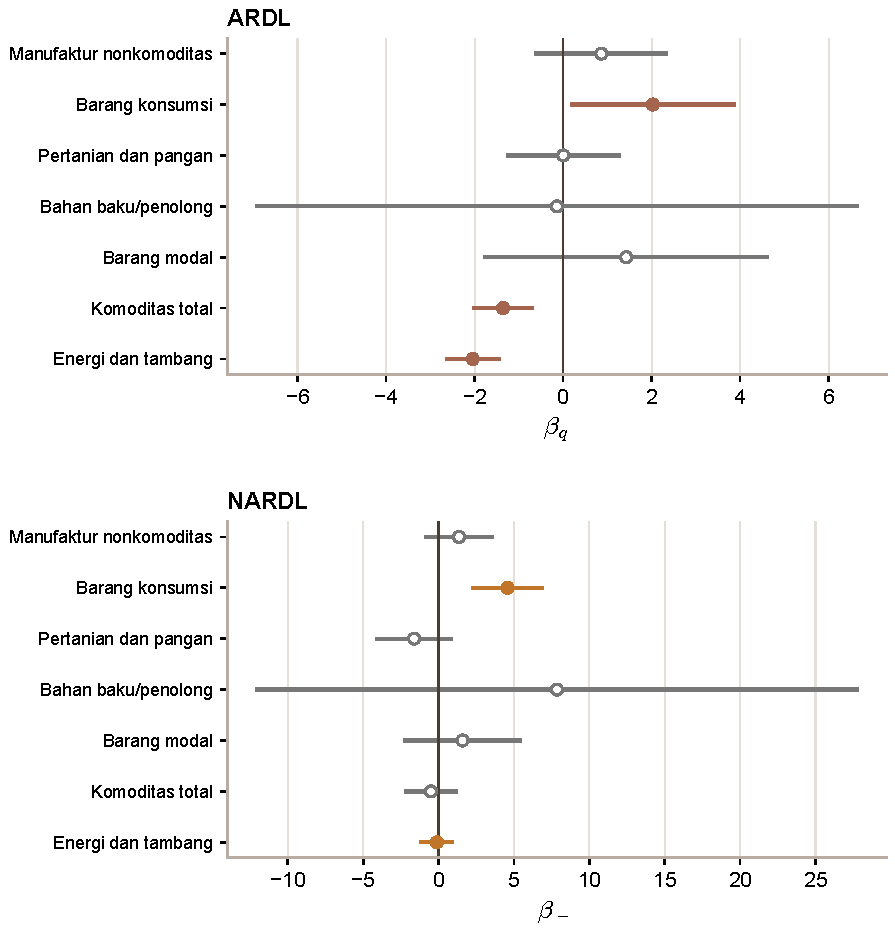
\includegraphics[width=\linewidth,height=.79\textheight,keepaspectratio]{assets/world_goods_forest.pdf}
\caption{Interval koefisien tujuh kelompok perdagangan Indonesia terhadap seluruh negara. Cokelat: syarat level dan diagnostik; emas: level dengan catatan diagnostik; simbol kosong: level belum lengkap. Status tidak menyatakan signifikansi koefisien dengan sendirinya.}\label{fig:goodsforest}
\end{figure}

Pada model linier, komoditas total dan energi/tambang memberikan koefisien negatif yang signifikan, dengan dukungan level serta diagnostik menurut aturan utama. Barang konsumsi mengarah positif dengan signifikansi nominal, tetapi nilai BH sekitar 0,124. Pada model nonlinear, barang konsumsi serta energi/tambang memenuhi syarat level, namun mempunyai catatan diagnostik. Tidak ada NARDL kelompok agregat yang sekaligus lolos syarat level dan seluruh penyaringan diagnostik yang digunakan.

\subsection{Komoditas total dan energi/tambang}
Koefisien ARDL komoditas total sekitar $-1,355$, dengan probabilitas nominal di bawah 0,001 dan BH sekitar 0,0037. Energi/tambang mempunyai koefisien sekitar $-2,040$ dengan probabilitas yang lebih kecil. Dengan orientasi apresiasi pada kurs, depresiasi berarti penurunan regressor; dikalikan koefisien negatif, perubahan outcome impor/ekspor mengarah positif atau memburuk.

Hasil ini relevan bagi hipotesis bahwa depresiasi tidak selalu memberi perbaikan. Namun ia belum mengidentifikasi apakah penyebabnya berada pada harga ekspor, volume, impor atau komposisi. Kelompok energi/tambang adalah bagian komoditas total, sehingga kedua temuan tidak boleh dihitung sebagai dua konfirmasi yang independen. Sebagian nilai perdagangan dan kejutan yang mereka alami sama.

NARDL memberikan gambaran lebih lemah untuk efek depresiasi kelompok tersebut. Koefisien komoditas total sekitar $-0,504$ tidak signifikan dan joint-X belum menolak meskipun F/t bounds menolak. Energi/tambang mempunyai koefisien depresiasi sekitar $-0,112$ yang tidak signifikan; hubungan level didukung, tetapi ada catatan heteroskedastisitas. Pada kelompok energi/tambang, Wald asimetri signifikan tidak berarti koefisien depresiasinya juga signifikan. Perbedaan koefisien kedua arah dan pengujian satu koefisien terhadap nol adalah pertanyaan berbeda.

\begin{figure}[!htbp]\centering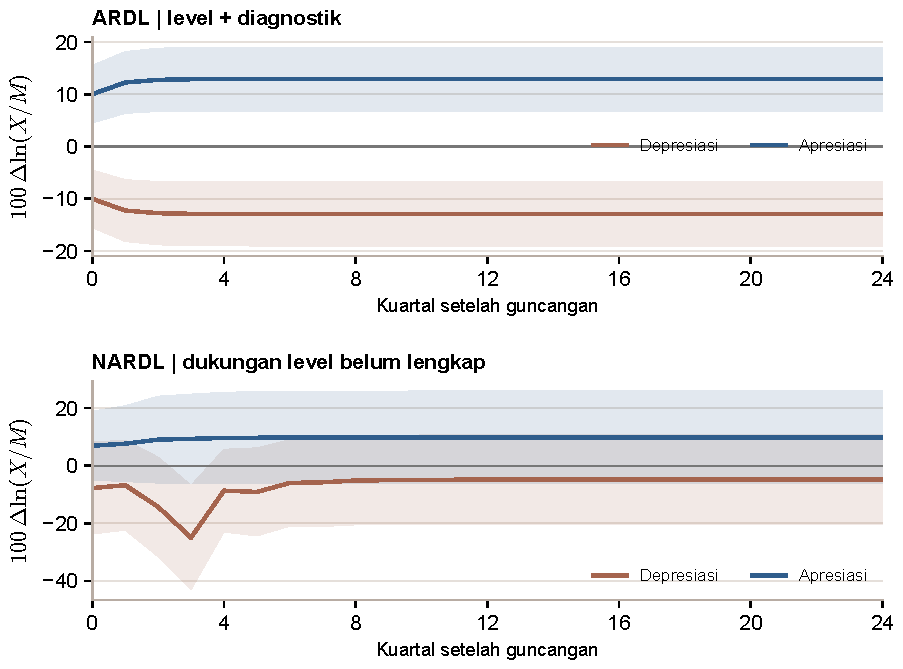
\includegraphics[width=\linewidth]{assets/response_TYPE_WLD_commodity.pdf}
\caption{Respons komoditas total Indonesia--seluruh dunia. ARDL mengarah pada pemburukan saat depresiasi; NARDL memberi ketepatan serta dukungan level yang berbeda. Band nominal pointwise 95\%.}\label{fig:commodity}
\end{figure}

\subsection{Manufaktur nonkomoditas}
ARDL manufaktur nonkomoditas memberi koefisien sekitar 0,865 dan NARDL koefisien depresiasi sekitar 1,358. Kedua probabilitas nominal berada di atas lima persen. Dukungan hubungan level juga belum lengkap. Karena itu, tanda titik positif belum dapat dipakai menyatakan bahwa manufaktur terbukti lebih diuntungkan oleh depresiasi dibandingkan komoditas.

Kegagalan menolak efek nol tidak sama dengan bukti bahwa efeknya kecil secara ekonomi. Interval harus cukup sempit untuk membedakan efek yang dianggap kecil dari yang relevan, dengan batas yang ditetapkan dan dijustifikasi. Run ini belum melakukan uji ekuivalensi tersebut. Membandingkan koefisien satu kelompok yang signifikan dengan kelompok lain yang tidak signifikan juga belum merupakan uji formal selisih dua koefisien.

\subsection{Konsumsi, pertanian, bahan baku/penolong dan modal}
NARDL konsumsi memberikan koefisien depresiasi sekitar 4,580, signifikan nominal maupun BH. Namun ada korelasi serial, heteroskedastisitas, RESET dan CUSUMSQ yang ditolak. Koefisien yang besar tidak dapat dipisahkan dari masalah spesifikasi ini. ARDL konsumsi lolos penyaringan utama dan memperlihatkan pola J pada titik, tetapi probabilitas BH-nya melewati lima persen dan dua fase belum terpisah kuat pada interval.

Pertanian/pangan dan modal memberikan contoh lain mengapa F/t tidak dibaca sendirian. Pada NARDL keduanya menolak no-level relation menurut F/t, tetapi joint-X belum mendukung. Bahan baku/penolong memberi interval yang sangat lebar dan catatan CUSUM, sementara syarat F/t juga belum lengkap. Tambahan parameter dan variasi regressor yang terbatas dapat mengurangi ketepatan. Koefisien besar pada kelompok ini karena itu tidak diperlakukan sebagai elastisitas yang telah mapan.

Klasifikasi penggunaan barang tidak mengaktifkan kembali hipotesis kandungan input impor. Besarnya koefisien bahan baku/penolong belum menjelaskan ketergantungan eksportir pada bahan asing. Data yang dibutuhkan untuk mekanisme itu berbeda dari pengelompokan perdagangan berdasarkan penggunaan barang.

\subsection{Perbedaan antara kelompok agregat dan kelompok bilateral}
Pertanian Indonesia--Tiongkok memberi contoh arah pemburukan yang lebih terukur pada NARDL. Koefisien depresiasinya sekitar $-2,037$, dengan probabilitas nominal sekitar 0,0016 dan BH sekitar 0,0148, serta memenuhi syarat level dan diagnostik utama. Temuan itu berlaku pada rasio neraca pertanian dengan Tiongkok dalam window model. Ia tidak menetapkan bahwa seluruh ekspor pertanian Indonesia menurun akibat depresiasi.

Sebaliknya, modal Indonesia--Korea dan konsumsi Indonesia--AS memberikan contoh urutan J yang lebih jelas pada band pointwise: ada bagian awal di bawah nol dan akhir horizon di atas nol. Kedua spesifikasi lolos penyaringan level dan diagnostik utama. Hal ini memperlihatkan bahwa bukti di dalam data tidak hanya mengarah pada satu sisi hipotesis. Tetap diperlukan kehati-hatian karena pencarian horizon, pemilihan AIC dan pengujian banyak kelompok belum tercakup dalam uji simultan seluruh jalur.

\begin{figure}[!htbp]\centering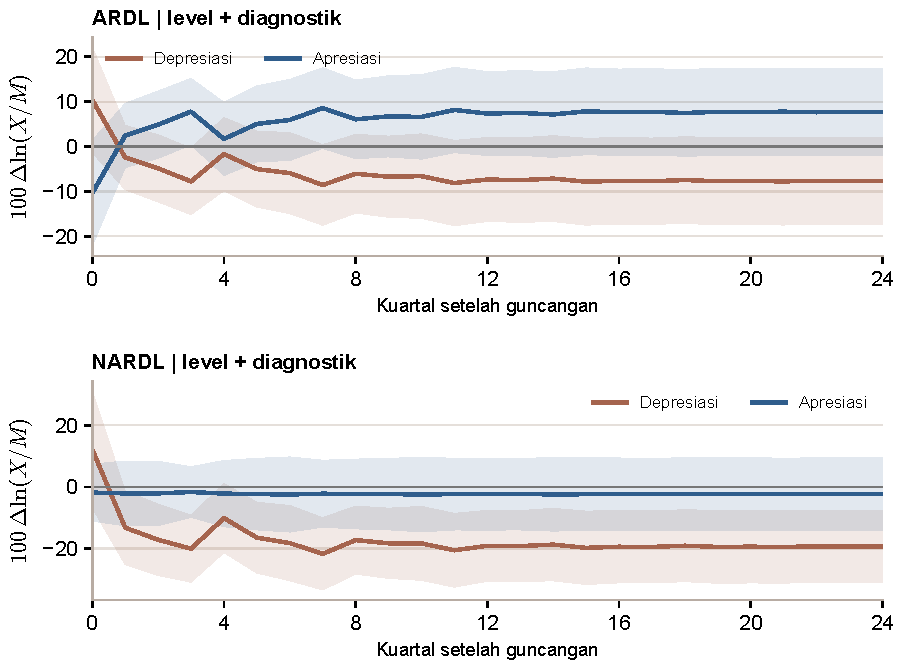
\includegraphics[width=\linewidth]{assets/response_TYPE_CHN_agriculture.pdf}
\caption{Pertanian Indonesia--Tiongkok sebagai contoh perbedaan hasil linier dan nonlinear. Positif berarti perbaikan rasio ekspor/impor.}\label{fig:chinaagri}
\end{figure}

Pada modal Korea, probabilitas BH koefisien depresiasi sekitar 0,104, sedangkan konsumsi AS sekitar 0,0027. Kejelasan dua fase pada band pointwise karena itu belum berarti semua koreksi pengujian berganda telah dilalui oleh keduanya.

\begin{figure}[!htbp]\centering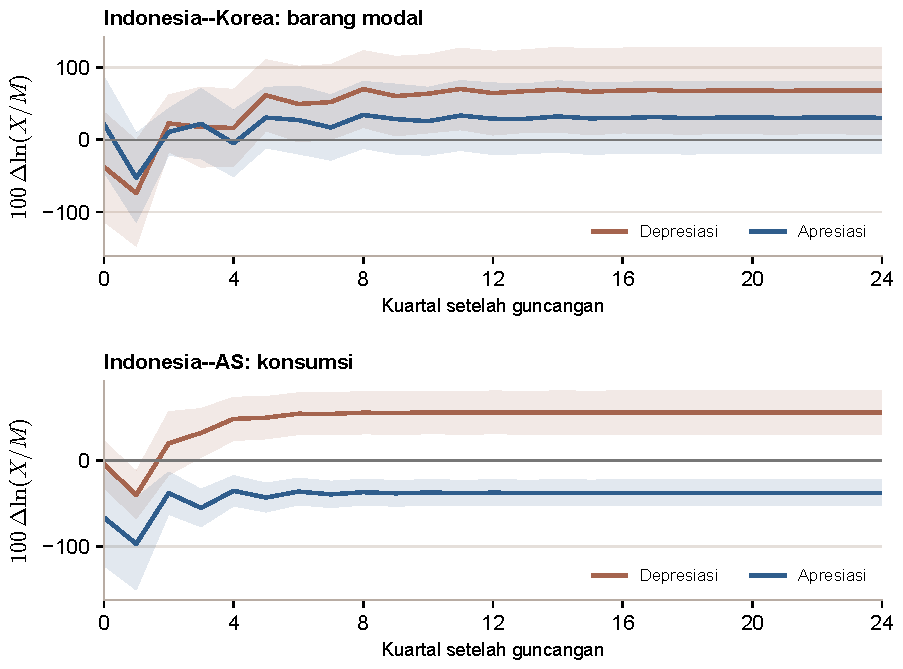
\includegraphics[width=\linewidth]{assets/J_examples.pdf}
\caption{Dua contoh NARDL dengan fase awal dan akhir yang lebih terpisah pada band pointwise: modal Indonesia--Korea dan konsumsi Indonesia--AS. Pemilihan horizon serta seleksi model belum tercakup dalam uji simultan.}\label{fig:Jexamples}
\end{figure}

Kesimpulan kelompok bersifat heterogen dan bergantung spesifikasi. Data memberi alasan melampaui satu angka agregat, tetapi belum mendukung penggantian generalisasi bahwa depresiasi selalu menguntungkan dengan generalisasi lain bahwa komoditas selalu tidak responsif atau selalu dirugikan.

\clearpage\section{Diagnostik, sensitivitas dan kekuatan bukti}\label{sec:diagnostics}
\subsection{Penyaringan level dan diagnostik dibedakan}
Sebanyak 95 dari 176 model utama menolak hipotesis tidak ada hubungan level menurut F dan t pada lima persen. Setelah joint-X, akar, risiko integrasi orde dua dan derajat bebas dipertimbangkan, 62 memenuhi syarat level operasional. Sebanyak 28 sekaligus tidak ditolak pada penyaringan residual dan stabilitas yang digunakan. Angka terakhir tidak berarti hanya 28 model benar, atau bahwa model lain tidak memberi informasi. Ia menunjukkan konsekuensi satu himpunan aturan yang dibuat transparan.

Diagnostik meliputi Breusch--Godfrey untuk korelasi serial, Breusch--Pagan untuk heteroskedastisitas, RESET untuk indikasi bentuk fungsi, Jarque--Bera untuk normalitas, ARCH, serta CUSUM dan CUSUMSQ untuk stabilitas. Normalitas bukan syarat universal konsistensi OLS, dan penolakan normalitas tidak mempunyai arti yang sama dengan penolakan kestabilan parameter. Penggabungan semuanya sebagai flag bersih adalah pilihan penyaringan yang konservatif. Pembaca tetap perlu melihat jenis penolakan, bukan hanya satu status akhir.

Tidak ditolaknya diagnostik juga bukan bukti bahwa asumsi pasti benar. Daya uji dapat rendah pada sampel kecil atau ketika banyak parameter diestimasi. Hasil residual yang tampak baik belum menyelesaikan endogenitas kurs, pemilihan variabel, maupun salah pengukuran. Probabilitas kecil menunjukkan ketidakcocokan data dengan hipotesis nol di bawah asumsi uji, bukan probabilitas bahwa hipotesis nol itu benar.

\subsection{Stabilitas dan pemeriksaan independen}
CUSUM utama diekspor langsung melalui \texttt{estat sbcusum} dari UECM dengan lag dan sampel terpilih \cite{stata}. Maksimum lintasan direkonsiliasi terhadap statistik tersimpan untuk seluruh 176 model utama. Pada matriks awal full rank, konstruksi independen juga diwajibkan cocok dalam toleransi numerik.

Dua model kelompok Australia, modal dan konsumsi NARDL, mempunyai matriks awal yang belum full rank. Prosedur independen menunda inisialisasi sampai full rank, sehingga berbeda dari Stata. Lintasan resmi Stata dipertahankan, perbedaannya dicatat, dan kedua model diberi caveat. Kasus tersebut berbeda dari model bilateral Australia yang dibahas pada hasil utama.

CUSUMSQ memakai referensi Gaussian Monte Carlo dengan 19.999 simulasi dan seed tetap. Band simultan referensinya hanya berlaku dalam konstruksi diagnostik tersebut, tidak mengubah band respons dinamis menjadi simultan. Perkiraan probabilitas Monte Carlo bersifat aproksimasi dan tidak diklaim sebagai tabel persis paper. Agregat perdagangan Indonesia memberi catatan CUSUMSQ, sedangkan Australia tidak ditolak dalam penyaringan utama.

\begin{figure}[!htbp]\centering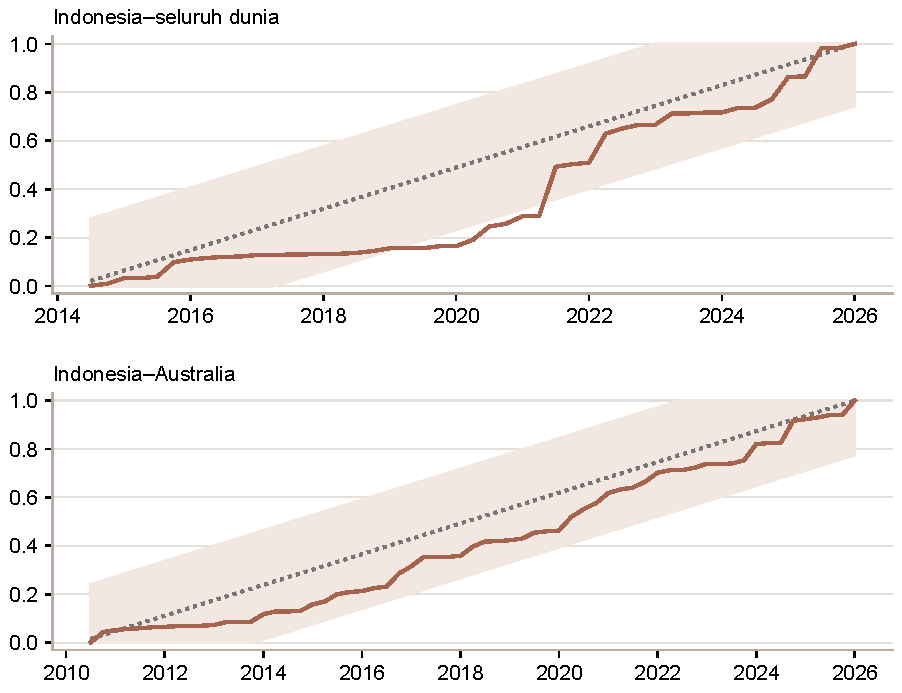
\includegraphics[width=\linewidth]{assets/stability.pdf}
\caption{CUSUMSQ NARDL agregat Indonesia dan Indonesia--Australia. Area menunjukkan band referensi simulasi; garis titik adalah lintasan ekspektasi. Ini diagnostik stabilitas, bukan band ketidakpastian efek kurs.}\label{fig:stability}
\end{figure}

Seluruh model juga diperiksa melalui ekuivalensi residual persamaan level dan ECM serta prediksi OLS independen. Pemeriksaan numerik itu lulus. Maknanya adalah bahwa perhitungan yang dilakukan konsisten, bukan bahwa semua asumsi ekonomi dan inferensinya telah terbukti.

\subsection{Ketahanan terhadap lag, harga dan sumber}
Pada ARDL, arah negatif komoditas total dan energi/tambang tetap muncul ketika cap dipersempit menjadi dua serta ketika BCOM ditambahkan. Namun beberapa varian memiliki catatan diagnostik. NARDL belum memberikan koefisien depresiasi yang signifikan pada kelompok ini, dan dukungan level dapat berubah menurut cap. Ketahanan tanda pada subset model linier karena itu tidak cukup untuk menyatakan hasil tahan terhadap seluruh spesifikasi.

\begin{table}[!htbp]\centering
\caption{Pembanding ARDL komoditas Indonesia--seluruh dunia}
{\small\setlength{\tabcolsep}{3pt}\renewcommand{\arraystretch}{1.15}
\begin{tabular}{p{0.08\linewidth}p{0.2\linewidth}p{0.08\linewidth}p{0.2\linewidth}p{0.15\linewidth}p{0.12\linewidth}}
\toprule
\textbf{Kel.} & \textbf{Varian} & \textbf{N} & \textbf{Koef. kurs} & \textbf{p} & \textbf{Status}\\
\midrule
G6 & Utama & 61 & -1,355 & \(<0{,}001\) & L+D\\
G6 & Cap 2 & 63 & -1,536 & \(<0{,}001\) & L+D\\
G6 & BCOM & 61 & -1,378 & \(<0{,}001\) & L\\
G7 & Utama & 61 & -2,040 & \(<0{,}001\) & L+D\\
G7 & Cap 2 & 63 & -2,222 & \(<0{,}001\) & L\\
G7 & BCOM & 61 & -2,305 & \(<0{,}001\) & L\\
\bottomrule
\end{tabular}
}\label{tab:sens}
\end{table}

BCOM adalah indeks luas, bukan harga setiap HS-6. Ia dapat bergerak bersama aktivitas global, harga energi dan kondisi keuangan yang juga berkaitan dengan kurs. Memasukkannya sebagai regressor membantu menilai apakah hasil berubah ketika satu kontrol harga ditambahkan; ia belum mengidentifikasi saluran kausal harga global. Interval klasik pada model yang menolak heteroskedastisitas juga perlu dinilai ulang sebelum digunakan untuk klaim yang kuat.

Sensitivitas lain meliputi perluasan window agregat 2006+, WPI India, dan keluarga FX GEM untuk Thailand, Vietnam dan Korea. Perubahan sumber dapat mengubah konsep harga, nilai kurs, dan kelengkapan window sekaligus. Sebagian perbandingan itu belum merupakan eksperimen satu perubahan pada sampel identik. Semua 340 sensitivitas dipertahankan dalam lampiran agar pembaca dapat melihat hasil yang tidak searah dengan baseline.

Tiga model NARDL India dengan BCOM tidak memiliki inferensi bounds finite-sample yang tersedia pada implementasi: komoditas total, energi/tambang, dan bahan baku/penolong. Ketiganya mempunyai 49 observasi dan 25--27 parameter. Koefisiennya tetap diestimasi; status bounds adalah tidak tersedia dan tidak dipakai sebagai dukungan level. Ketidaktersediaan inferensi tidak diubah menjadi keputusan menerima atau menolak kointegrasi.

\subsection{Bentuk J pada titik dan dukungan dua fase}
Agar penilaian grafik dapat ditelusuri, pemeriksaan titik dalam deck dan naskah menggunakan
\begin{equation}
 \min_{0\le h\le4}R_h^{J,-}<0,\qquad
 \frac{1}{9}\sum_{h=16}^{24}R_h^{J,-}>0.
 \label{eq:jvisual}
\end{equation}
Ini definisi visual-operasional: setidaknya satu pemburukan pada tahun pertama, termasuk impact, dan rerata positif pada bagian akhir horizon. Definisi tersebut bukan uji formal J-curve paper, bukan long-run limit, dan tidak dipraregistrasikan sebagai desain inferensi.

\begin{table}[!htbp]\centering
\caption{Pola J pada seluruh model utama}
{\small\setlength{\tabcolsep}{3pt}\renewcommand{\arraystretch}{1.15}
\begin{tabular}{p{0.18\linewidth}p{0.12\linewidth}p{0.15\linewidth}p{0.21\linewidth}p{0.23\linewidth}}
\toprule
\textbf{Model} & \textbf{Seri} & \textbf{J titik} & \textbf{J + L+D} & \textbf{Dua fase CI}\\
\midrule
ARDL & 88 & 10 & 1 & 0\\
NARDL & 88 & 24 & 5 & 2\\
\bottomrule
\end{tabular}
}\label{tab:j}
\end{table}

Pada titik estimasi terdapat sepuluh pola J ARDL dan 24 NARDL. Setelah syarat level dan diagnostik diperiksa, tersisa satu ARDL dan lima NARDL. Syarat tambahan bahwa sebagian fase awal mempunyai batas atas di bawah nol dan kuartal ke-24 mempunyai batas bawah di atas nol menghasilkan nol ARDL dan dua NARDL. Dua NARDL itu adalah modal Korea dan konsumsi AS.

Pencarian salah satu horizon awal masih menimbulkan pengujian berganda, sehingga dua kasus tersebut tidak menjadi uji simultan dua fase yang sah. Jumlah model yang bertumpang tindih juga tidak dapat dibaca sebagai frekuensi kejadian J-curve di populasi. Yang dapat dinyatakan adalah bahwa bukti interval lebih terbatas daripada kesan visual titiknya.

\subsection{Mengapa ARDL dan NARDL dapat berbeda}
NARDL menambah parameter dan membagi variasi kurs ke dua partial sums yang dapat berkorelasi kuat dengan tren aktivitas ekonomi. Ketepatan efek satu arah dapat turun, sementara hubungan yang dipaksakan simetris pada ARDL menjadi lebih presisi. AIC juga dapat memilih lag yang berbeda. Perbedaan keduanya tidak otomatis membuktikan salah satu model benar.

Pemilihan model sebaiknya tidak hanya didasarkan pada tanda yang disukai. Relevansi ekonomi, kesesuaian definisi, dukungan level, ketepatan, diagnostik dan sensitivitas harus diperiksa bersama. Pada data yang ada, ketidaksepakatan antara hasil komoditas linier dan nonlinear merupakan bagian dari temuan, bukan gangguan yang dihapus dari narasi.

\clearpage\section{Pembahasan dan kesimpulan}\label{sec:discussion}
\subsection{Apa arti hasil bagi hipotesis awal}
Hasil belum memberi dasar bagi pernyataan bahwa depresiasi merupakan jaminan perbaikan neraca Indonesia. Agregat utama belum mendukung hubungan level yang kuat. Pada disaggregasi, terdapat pasar atau kelompok yang mengarah pada perbaikan dan terdapat yang mengarah pada pemburukan. Sebagian bukti lebih kuat menurut penyaringan yang dipakai, tetapi kesimpulannya tidak seragam antarspesifikasi.

Temuan linier komoditas total serta energi/tambang relevan bagi hipotesis awal. Arah negatif tetap terlihat pada beberapa pembanding, sehingga hubungan tersebut tidak hanya muncul pada satu tabel baseline. Namun NARDL belum memberikan konfirmasi setara, dan beberapa sensitivitas menolak diagnostik. Oleh karena itu, naskah tidak menyimpulkan bahwa karakter komoditas telah terbukti sebagai penyebab arah negatif tersebut.

Pangsa komoditas membantu menjelaskan mengapa agregasi barang layak dilakukan. Ia belum menghubungkan secara kausal harga internasional dengan koefisien kurs. Regresi tambahan BCOM pun belum memisahkan harga ekspor, harga impor, volume dan kondisi permintaan. Klaim mekanisme memerlukan pengukuran serta desain identifikasi yang berbeda dari sekadar menambahkan satu indeks kontrol.

\subsection{Batas penafsiran ekspor, neraca dan ketidakpekaan}
Outcome rasio neraca memberi informasi relatif. Penurunan impor yang lebih cepat daripada ekspor dapat menghasilkan perbaikan tanpa pertumbuhan ekspor. Sebaliknya, ekspor dapat meningkat tetapi impor naik lebih cepat, sehingga rasio memburuk. Menerjemahkan hasil menjadi pernyataan ekspor saja akan melewati informasi yang tersedia. Untuk hipotesis khusus ekspor, persamaan ekspor terpisah perlu dinilai dengan regressor dan identifikasi yang sesuai.

Ketidakpekaan terhadap kurs juga merupakan klaim yang lebih kuat daripada tidak signifikan. Interval lebar dapat memuat efek negatif maupun positif yang besar. Hasil seperti itu terutama menunjukkan ketidakpastian. Uji ekuivalensi akan memerlukan batas pengaruh yang dianggap kecil secara ekonomi dan justifikasi atas batas tersebut. Run ini belum melaksanakannya.

Heterogenitas antarbarang perlu diuji secara langsung apabila menjadi klaim utama. Membandingkan bintang pada dua regresi belum menguji kesamaan koefisien keduanya. Perbedaan window, korelasi residual, dan tumpang tindih kategori juga harus dipertimbangkan dalam desain uji. Bukti deskriptif dan matriks koefisien dalam PPT berfungsi memetakan masalah itu, tidak menggantikannya.

\subsection{Keterbatasan yang paling menentukan}
Pertama, revisi HS per sel belum diketahui. Konsensus lintas korespondensi menjaga agar kelas ambigu tidak dipaksakan, tetapi mengubah kode menjadi seri produk yang benar-benar sebanding sepanjang waktu masih memerlukan harmonisasi. Perubahan cakupan klasifikasi dapat berkaitan dengan komposisi kelompok dan memengaruhi rasio ekspor/impor.

Kedua, ketersediaan CPI, FX dan GDP menghasilkan sampel tidak seragam. India memiliki observasi lebih sedikit; celah AS dan Vietnam memotong window utama. Perbandingan lintas mitra karena itu mengandung perbedaan pengalaman ekonomi yang diamati. Proksi aktivitas agregat juga hanya merepresentasikan sepuluh mitra dengan bobot tetap.

Ketiga, nilai perdagangan belum dipisahkan ke harga dan volume serta belum disesuaikan musiman. Kejutan harga global dapat mengubah nilai dua arus meskipun volume tidak merespons. Pola musiman yang berbeda antara perdagangan dan GDP penyedia juga dapat berpengaruh. Diagnostik memberi petunjuk, tetapi tidak menentukan satu perbaikan yang pasti.

Keempat, kurs dapat merespons neraca dan kejutan makro yang sama. Lag membantu menggambarkan waktu penyesuaian, tetapi tidak otomatis membuat regressor eksogen. Tidak ada instrumen, kejutan kebijakan teridentifikasi atau rancangan kausal lain dalam run ini. Istilah hubungan kondisional karena itu lebih sesuai daripada efek kebijakan yang telah terisolasi.

Kelima, 516 estimasi menciptakan ruang besar untuk pencarian hasil. BH hanya diterapkan dalam keluarga utama tertentu dan belum menyelesaikan seleksi lag maupun semua perbandingan sensitivitas. Pelaporan lengkap merupakan langkah transparansi, bukan koreksi penuh seluruh ketidakpastian tersebut.

\subsection{Pengembangan penelitian yang paling dekat dengan pertanyaan}
Prioritas empiris berikutnya adalah menyelaraskan definisi dan sampel sebelum memperbanyak model. Harmonisasi HS dan dokumentasi cakupan akan memperkuat komposisi barang. Perbandingan pada window yang sama akan membantu memisahkan heterogenitas ekonomi dari perbedaan periode. Pemeriksaan musiman dan spesifikasi residual perlu mengikuti persoalan yang terlihat, dengan inferensi yang sesuai bila asumsi varians atau korelasi ditolak.

Bila fokus akhirnya adalah ekspor, data kuantitas atau ukuran harga yang sebanding akan membantu membedakan respons nilai dari volume. Model ekspor terpisah dapat menjawab pertanyaan yang tidak dapat dijawab rasio neraca. Estimasi tiap HS-6 juga memerlukan penanganan nol, perubahan kode, kecukupan sampel dan pengujian berganda; tidak semua seri produk dapat langsung dimasukkan ke model log yang sama. Hipotesis input impor tetap berada di luar run ini dan memerlukan sumber data lain.

\subsection{Kesimpulan}
Analisis perdagangan Indonesia menunjukkan bahwa satu koefisien agregat belum merangkum seluruh pengalaman pasar dan barang. Australia dan Malaysia memberikan dukungan lebih baik pada NARDL bilateral, dengan ketahanan signifikansi yang berbeda setelah BH. ARDL komoditas total serta energi/tambang mengarah pada pemburukan saat depresiasi, tetapi dukungan nonlinear dan diagnostik pembanding belum seragam. Pola J terlihat pada sebagian titik estimasi, sementara dukungan kedua fase pada interval lebih jarang.

Kesimpulan yang dapat dipertahankan adalah bahwa manfaat depresiasi terhadap neraca tidak terukur secara seragam dalam spesifikasi yang diperiksa. Penelitian ini belum membuktikan bahwa depresiasi selalu merugikan, bahwa komoditas pasti tidak sensitif, atau bahwa harga global telah menjadi penyebab yang teridentifikasi. Pembedaan antara hasil, kelayakan model dan penafsiran mekanisme merupakan dasar untuk melanjutkan penelitian dengan klaim yang lebih tepat.

\clearpage\begin{thebibliography}{99}
\addcontentsline{toc}{section}{Daftar pustaka}
\bibitem{bahmani}
Bahmani-Oskooee, M. dan Fariditavana, H. (2016; terbit daring 2015).
Nonlinear ARDL Approach and the J-Curve Phenomenon.
\emph{Open Economies Review}, 27(1), 51--70.
\url{https://doi.org/10.1007/s11079-015-9369-5}.
Paper lengkap yang diberikan pengguna tersedia pada referensi proyek.

\bibitem{pss}
Pesaran, M. H., Shin, Y. dan Smith, R. J. (2001).
Bounds testing approaches to the analysis of level relationships.
\emph{Journal of Applied Econometrics}, 16(3), 289--326.
\url{https://doi.org/10.1002/jae.616}.

\bibitem{shin}
Shin, Y., Yu, B. dan Greenwood-Nimmo, M. (2014).
Modelling Asymmetric Cointegration and Dynamic Multipliers in a Nonlinear ARDL Framework.
Dalam \emph{Festschrift in Honor of Peter Schmidt}, 281--314.
Springer. \url{https://doi.org/10.1007/978-1-4899-8008-3_9}.

\bibitem{ks}
Kripfganz, S. dan Schneider, D. C. (2023).
ardl: Estimating autoregressive distributed lag and equilibrium correction models.
\emph{The Stata Journal}, 23(4), 983--1019.
\url{https://doi.org/10.1177/1536867X231212434}.

\bibitem{bh}
Benjamini, Y. dan Hochberg, Y. (1995).
Controlling the False Discovery Rate: A Practical and Powerful Approach to Multiple Testing.
\emph{Journal of the Royal Statistical Society: Series B}, 57(1), 289--300.
\url{https://doi.org/10.1111/j.2517-6161.1995.tb02031.x}.

\bibitem{bec}
United Nations Statistics Division (2018).
\emph{Classification by Broad Economic Categories, Revision 5},
ST/ESA/STAT/SER.M/53/Rev.5.
\url{https://unstats.un.org/unsd/trade/classifications/bec.asp}.
Manual dan korespondensi disimpan dalam referensi proyek.

\bibitem{unsdcorr}
United Nations Statistics Division (2022).
\emph{HS--SITC--BEC Correlations dan korespondensi antar revisi HS}.
\url{https://unstats.un.org/unsd/classifications/Econ/}.
File sumber lokal: \texttt{unsd\_correlations\_2022.xlsx}
dan korespondensi HS--SITC dalam folder referensi klasifikasi.

\bibitem{unctad}
UNCTAD (tanpa tahun; salinan lokal diakses 2026).
\emph{SITC Rev.3 Products: Special Groupings Hierarchy},
kelompok komoditas A11.
\url{https://unctadstat.unctad.org/EN/Classifications/DimSitcRev3Products_DsibSpecialGroupings_Hierarchy.pdf}.
Salinan lokal dan manifest unduhan dipertahankan untuk penelusuran.

\bibitem{stata}
StataCorp.
\emph{estat sbcusum: Cumulative sum test for parameter stability}.
Manual resmi Stata.
\url{https://www.stata.com/manuals/tsestatsbcusum.pdf}.

\bibitem{local}
Dokumentasi proyek Tio (2026).
Audit data HS-6, audit validitas makro, manifest sumber dan hasil estimasi.
Berkas lokal pada \path{input/reference/},
\path{output/diagnostics/data/} dan
\path{output/diagnostics/oskooee/}.
Audit cakupan negara pelapor: \path{output/presentation/scope_audit_indonesia.json}.
Statistik dan estimasi naskah menggunakan keluaran run 17 November 2026.
\end{thebibliography}

\clearpage\appendix\section{Panduan membaca tabel lengkap}\label{app:read}
Lampiran mempertahankan 176 model utama dan 340 sensitivitas, termasuk model yang belum mendukung level atau mempunyai catatan diagnostik. Kolom koefisien menggunakan $\beta_q$ pada ARDL dan $\beta_-$ pada NARDL. Dengan definisi kurs yang digunakan, koefisien positif mengarah pada perbaikan rasio neraca ketika depresiasi, sedangkan negatif mengarah pada pemburukan. Penafsiran itu tetap memerlukan kelayakan hubungan level.

\subsection{Kode pasar, kelompok, dan varian}
Negara pelapor semua tabel adalah Indonesia. \texttt{WLD} berarti seluruh negara mitra; \texttt{AUS}, \texttt{CHN}, \texttt{IND}, \texttt{JPN}, \texttt{KOR}, \texttt{MYS}, \texttt{SGP}, \texttt{THA}, \texttt{USA}, dan \texttt{VNM} adalah mitra yang sudah dibahas. G0 berarti seluruh barang pada cakupan pasar tersebut. G1--G7 mengikuti Tabel~\ref{tab:groups}.

Varian U adalah baseline maksimum empat lag level; L2 maksimum dua; P tambahan kontrol BCOM; W06 perluasan window agregat Indonesia 2006+; WPI memakai proksi harga WPI India; FX memakai keluarga kurs GEM alternatif. Perbedaan varian dapat melibatkan perubahan window atau konsep sumber. Tabel tidak menjadikan varian-varian tersebut sebagai eksperimen yang hanya berbeda satu unsur.

\subsection{Arti status}
\texttt{L+D} berarti syarat level dan penyaringan diagnostik yang digunakan terpenuhi. \texttt{L} berarti syarat level terpenuhi tetapi ada catatan diagnostik. Tanda -- berarti dukungan level lengkap belum terpenuhi atau inferensinya tidak tersedia. Model dengan tanda -- tetap dapat mempunyai koefisien nominal signifikan. Status tidak secara otomatis menentukan bahwa suatu efek berbeda dari nol.

Probabilitas BH hanya dihitung pada keluarga model utama. Kolom BH sensitivitas karena itu ditulis --. Probabilitas lebih kecil dari 0,001 dicetak sebagai $<0{,}001$, bukan sebagai nol persis. Jumlah observasi adalah sampel estimasi setelah lag, bukan jumlah bulan atau kuartal raw.

\subsection{Berkas yang memuat rincian lebih jauh}
Workbook \path{output/tables/oskooee/Oskooee_Results.xlsx} memuat seluruh koefisien, unit root, registry sampel dan status. \path{results_all_models.csv} serta \path{diagnostic_summary.csv} menyimpan probabilitas masing-masing diagnostik. Identitas model lengkap pada \path{assets/all_516_models_source.csv} memungkinkan tabel ringkas ini dipadankan dengan hasil Stata.

Atlas respons lengkap berada dalam PPT versi lengkap dan dipetakan melalui \path{model_response_slide_index.csv} pada folder presentasi. Paper memuat grafik terpilih untuk pendalaman, sedangkan tabel berikut mempertahankan semua estimasi numeriknya.

\clearpage\section{Seluruh 176 model utama}
\noindent Negara pelapor: Indonesia. Mitra \texttt{WLD} adalah seluruh negara. Kelompok dan status mengikuti Lampiran~\ref{app:read}. Koefisien belum menjadi hubungan jangka panjang yang mapan pada baris tanpa dukungan level.
{\footnotesize\setlength{\tabcolsep}{3pt}\renewcommand{\arraystretch}{1.15}
\begin{longtable}{p{0.075\linewidth}p{0.05\linewidth}p{0.09\linewidth}p{0.04\linewidth}p{0.05\linewidth}p{0.1\linewidth}p{0.085\linewidth}p{0.085\linewidth}p{0.075\linewidth}}
\toprule
\textbf{Mitra} & \textbf{Kel.} & \textbf{Model} & \textbf{N} & \textbf{Var.} & \textbf{Koef.} & \textbf{p} & \textbf{BH} & \textbf{Status}\\
\midrule
\endfirsthead
\toprule
\textbf{Mitra} & \textbf{Kel.} & \textbf{Model} & \textbf{N} & \textbf{Var.} & \textbf{Koef.} & \textbf{p} & \textbf{BH} & \textbf{Status}\\
\midrule
\endhead
\midrule\multicolumn{9}{r}{\footnotesize Bersambung ke halaman berikutnya}\\\endfoot
\bottomrule\endlastfoot
AUS & G3 & ARDL & 77 & U & -1,770 & 0,043 & 0,165 & --\\
AUS & G3 & NARDL & 77 & U & -3,345 & \(<0{,}001\) & 0,004 & L\\
AUS & G5 & ARDL & 77 & U & 4,002 & 0,120 & 0,307 & --\\
AUS & G5 & NARDL & 77 & U & 7,466 & 0,041 & 0,138 & --\\
AUS & G6 & ARDL & 77 & U & 1,701 & 0,008 & 0,103 & L+D\\
AUS & G6 & NARDL & 77 & U & 1,379 & 0,142 & 0,332 & L+D\\
AUS & G2 & ARDL & 77 & U & 0,704 & 0,316 & 0,544 & --\\
AUS & G2 & NARDL & 77 & U & 1,088 & 0,285 & 0,488 & --\\
AUS & G7 & ARDL & 77 & U & 3,265 & 0,026 & 0,121 & L\\
AUS & G7 & NARDL & 77 & U & 5,725 & 0,006 & 0,036 & L\\
AUS & G4 & ARDL & 77 & U & 1,608 & 0,024 & 0,121 & L\\
AUS & G4 & NARDL & 77 & U & 2,518 & 0,010 & 0,053 & L+D\\
AUS & G1 & ARDL & 77 & U & 0,919 & 0,460 & 0,656 & --\\
AUS & G1 & NARDL & 77 & U & 5,628 & 0,003 & 0,023 & --\\
AUS & G0 & ARDL & 77 & U & 2,084 & 0,002 & 0,021 & L+D\\
AUS & G0 & NARDL & 77 & U & 3,356 & \(<0{,}001\) & 0,004 & L+D\\
CHN & G3 & ARDL & 78 & U & -0,809 & 0,119 & 0,307 & L+D\\
CHN & G3 & NARDL & 78 & U & -2,036 & 0,002 & 0,015 & L+D\\
CHN & G5 & ARDL & 78 & U & 1,211 & 0,325 & 0,544 & L\\
CHN & G5 & NARDL & 78 & U & 0,595 & 0,764 & 0,842 & L\\
CHN & G6 & ARDL & 78 & U & -2,216 & 0,005 & 0,103 & L\\
CHN & G6 & NARDL & 78 & U & -3,458 & \(<0{,}001\) & 0,003 & L\\
CHN & G2 & ARDL & 78 & U & -0,569 & 0,567 & 0,752 & --\\
CHN & G2 & NARDL & 78 & U & -2,711 & 0,031 & 0,108 & L+D\\
CHN & G7 & ARDL & 78 & U & -1,924 & 0,101 & 0,300 & --\\
CHN & G7 & NARDL & 78 & U & -3,658 & 0,022 & 0,101 & L\\
CHN & G4 & ARDL & 78 & U & -3,291 & 0,046 & 0,168 & --\\
CHN & G4 & NARDL & 78 & U & -6,234 & 0,004 & 0,023 & --\\
CHN & G1 & ARDL & 78 & U & 0,300 & 0,878 & 0,955 & --\\
CHN & G1 & NARDL & 78 & U & 3,033 & 0,663 & 0,763 & --\\
CHN & G0 & ARDL & 78 & U & -1,886 & 0,059 & 0,148 & --\\
CHN & G0 & NARDL & 78 & U & -2,727 & 0,250 & 0,350 & --\\
IND & G3 & ARDL & 49 & U & 6,325 & 0,645 & 0,823 & --\\
IND & G3 & NARDL & 49 & U & -5,076 & 0,316 & 0,503 & L\\
IND & G5 & ARDL & 49 & U & 1,012 & 0,913 & 0,963 & --\\
IND & G5 & NARDL & 49 & U & 0,815 & 0,939 & 0,970 & --\\
IND & G6 & ARDL & 49 & U & 5,476 & 0,549 & 0,742 & --\\
IND & G6 & NARDL & 49 & U & -4,569 & 0,320 & 0,503 & L+D\\
IND & G2 & ARDL & 49 & U & 3,982 & 0,535 & 0,736 & --\\
IND & G2 & NARDL & 49 & U & -8,904 & 0,090 & 0,263 & L\\
IND & G7 & ARDL & 49 & U & 7,828 & 0,358 & 0,574 & --\\
IND & G7 & NARDL & 49 & U & -4,506 & 0,346 & 0,526 & L+D\\
IND & G4 & ARDL & 49 & U & 10,846 & 0,240 & 0,463 & --\\
IND & G4 & NARDL & 49 & U & 2,938 & 0,702 & 0,795 & --\\
IND & G1 & ARDL & 49 & U & -4,502 & 0,393 & 0,606 & --\\
IND & G1 & NARDL & 49 & U & -6,379 & 0,179 & 0,377 & --\\
IND & G0 & ARDL & 49 & U & 5,254 & 0,437 & 0,486 & --\\
IND & G0 & NARDL & 49 & U & -6,443 & 0,236 & 0,350 & --\\
JPN & G3 & ARDL & 78 & U & -0,075 & 0,925 & 0,963 & --\\
JPN & G3 & NARDL & 78 & U & -1,712 & 0,009 & 0,047 & --\\
JPN & G5 & ARDL & 78 & U & -3,068 & 0,075 & 0,241 & --\\
JPN & G5 & NARDL & 78 & U & -4,687 & 0,002 & 0,018 & --\\
JPN & G6 & ARDL & 78 & U & -1,771 & 0,009 & 0,103 & L\\
JPN & G6 & NARDL & 78 & U & -0,710 & 0,493 & 0,612 & L+D\\
JPN & G2 & ARDL & 78 & U & -0,718 & 0,337 & 0,553 & L\\
JPN & G2 & NARDL & 78 & U & -1,246 & 0,244 & 0,448 & L\\
JPN & G7 & ARDL & 78 & U & -2,107 & 0,016 & 0,119 & L\\
JPN & G7 & NARDL & 78 & U & -0,160 & 0,894 & 0,945 & L+D\\
JPN & G4 & ARDL & 78 & U & -2,347 & 0,021 & 0,121 & --\\
JPN & G4 & NARDL & 78 & U & -3,048 & 0,002 & 0,015 & --\\
JPN & G1 & ARDL & 78 & U & -1,171 & 0,166 & 0,375 & --\\
JPN & G1 & NARDL & 78 & U & -1,477 & 0,159 & 0,350 & --\\
JPN & G0 & ARDL & 78 & U & -2,106 & 0,017 & 0,058 & --\\
JPN & G0 & NARDL & 78 & U & -2,456 & 0,006 & 0,020 & --\\
KOR & G3 & ARDL & 78 & U & 1,449 & 0,056 & 0,187 & --\\
KOR & G3 & NARDL & 78 & U & 1,601 & 0,241 & 0,448 & --\\
KOR & G5 & ARDL & 78 & U & 1,416 & 0,420 & 0,622 & --\\
KOR & G5 & NARDL & 78 & U & 7,147 & 0,027 & 0,104 & L+D\\
KOR & G6 & ARDL & 78 & U & -0,370 & 0,857 & 0,955 & --\\
KOR & G6 & NARDL & 78 & U & 4,662 & 0,092 & 0,263 & --\\
KOR & G2 & ARDL & 78 & U & 7,941 & 0,118 & 0,307 & --\\
KOR & G2 & NARDL & 78 & U & 0,875 & 0,945 & 0,970 & --\\
KOR & G7 & ARDL & 78 & U & -0,712 & 0,773 & 0,910 & --\\
KOR & G7 & NARDL & 78 & U & 5,815 & 0,109 & 0,279 & --\\
KOR & G4 & ARDL & 78 & U & 0,887 & 0,652 & 0,823 & --\\
KOR & G4 & NARDL & 78 & U & 10,950 & 0,102 & 0,275 & --\\
KOR & G1 & ARDL & 78 & U & 1,747 & 0,055 & 0,187 & --\\
KOR & G1 & NARDL & 78 & U & 4,717 & 0,001 & 0,013 & --\\
KOR & G0 & ARDL & 78 & U & -0,074 & 0,944 & 0,944 & --\\
KOR & G0 & NARDL & 78 & U & 3,935 & 0,144 & 0,288 & --\\
MYS & G3 & ARDL & 78 & U & 0,338 & 0,803 & 0,922 & --\\
MYS & G3 & NARDL & 78 & U & 3,464 & 0,181 & 0,377 & --\\
MYS & G5 & ARDL & 78 & U & 0,178 & 0,751 & 0,904 & L+D\\
MYS & G5 & NARDL & 78 & U & 0,784 & 0,468 & 0,610 & L+D\\
MYS & G6 & ARDL & 78 & U & -1,290 & 0,088 & 0,270 & L+D\\
MYS & G6 & NARDL & 78 & U & 1,444 & 0,258 & 0,461 & L+D\\
MYS & G2 & ARDL & 78 & U & -0,746 & 0,695 & 0,850 & --\\
MYS & G2 & NARDL & 78 & U & 4,491 & 0,068 & 0,219 & --\\
MYS & G7 & ARDL & 78 & U & -1,376 & 0,116 & 0,307 & L+D\\
MYS & G7 & NARDL & 78 & U & 1,117 & 0,483 & 0,610 & L+D\\
MYS & G4 & ARDL & 78 & U & -0,645 & 0,408 & 0,617 & --\\
MYS & G4 & NARDL & 78 & U & 1,176 & 0,309 & 0,503 & --\\
MYS & G1 & ARDL & 78 & U & 0,285 & 0,845 & 0,955 & --\\
MYS & G1 & NARDL & 78 & U & 1,939 & 0,406 & 0,578 & --\\
MYS & G0 & ARDL & 78 & U & -0,716 & 0,081 & 0,163 & L\\
MYS & G0 & NARDL & 78 & U & 1,346 & 0,024 & 0,059 & L+D\\
SGP & G3 & ARDL & 78 & U & 5,982 & 0,027 & 0,121 & --\\
SGP & G3 & NARDL & 78 & U & 4,941 & 0,092 & 0,263 & --\\
SGP & G5 & ARDL & 78 & U & -0,469 & 0,669 & 0,831 & --\\
SGP & G5 & NARDL & 78 & U & -1,303 & 0,470 & 0,610 & --\\
SGP & G6 & ARDL & 78 & U & -1,192 & 0,025 & 0,121 & --\\
SGP & G6 & NARDL & 78 & U & -0,701 & 0,483 & 0,610 & --\\
SGP & G2 & ARDL & 78 & U & 2,616 & 0,325 & 0,544 & L\\
SGP & G2 & NARDL & 78 & U & -0,102 & 0,985 & 0,991 & --\\
SGP & G7 & ARDL & 78 & U & -1,383 & 0,016 & 0,119 & --\\
SGP & G7 & NARDL & 78 & U & -0,709 & 0,504 & 0,617 & --\\
SGP & G4 & ARDL & 78 & U & 0,424 & 0,604 & 0,788 & --\\
SGP & G4 & NARDL & 78 & U & -2,032 & 0,022 & 0,101 & L\\
SGP & G1 & ARDL & 78 & U & 0,007 & 0,994 & 0,994 & --\\
SGP & G1 & NARDL & 78 & U & -1,544 & 0,308 & 0,503 & --\\
SGP & G0 & ARDL & 78 & U & -0,451 & 0,432 & 0,486 & --\\
SGP & G0 & NARDL & 78 & U & -0,262 & 0,810 & 0,810 & --\\
THA & G3 & ARDL & 78 & U & 1,906 & 0,216 & 0,442 & --\\
THA & G3 & NARDL & 78 & U & 3,848 & 0,155 & 0,350 & L\\
THA & G5 & ARDL & 78 & U & -1,027 & 0,433 & 0,629 & --\\
THA & G5 & NARDL & 78 & U & 2,593 & 0,355 & 0,526 & --\\
THA & G6 & ARDL & 78 & U & 1,047 & 0,137 & 0,341 & --\\
THA & G6 & NARDL & 78 & U & 3,454 & 0,024 & 0,104 & --\\
THA & G2 & ARDL & 78 & U & 2,543 & 0,015 & 0,119 & L\\
THA & G2 & NARDL & 78 & U & 0,354 & 0,896 & 0,945 & --\\
THA & G7 & ARDL & 78 & U & -0,592 & 0,270 & 0,496 & --\\
THA & G7 & NARDL & 78 & U & 0,755 & 0,594 & 0,703 & --\\
THA & G4 & ARDL & 78 & U & 1,063 & 0,031 & 0,124 & L+D\\
THA & G4 & NARDL & 78 & U & -1,568 & 0,124 & 0,309 & L+D\\
THA & G1 & ARDL & 78 & U & 1,001 & 0,218 & 0,442 & --\\
THA & G1 & NARDL & 78 & U & 0,564 & 0,766 & 0,842 & --\\
THA & G0 & ARDL & 78 & U & 1,180 & 0,006 & 0,031 & L\\
THA & G0 & NARDL & 78 & U & 0,950 & 0,280 & 0,350 & L\\
USA & G3 & ARDL & 75 & U & -0,836 & 0,017 & 0,119 & L+D\\
USA & G3 & NARDL & 75 & U & 0,622 & 0,278 & 0,487 & L+D\\
USA & G5 & ARDL & 75 & U & 1,166 & 0,780 & 0,910 & --\\
USA & G5 & NARDL & 75 & U & 4,530 & 0,434 & 0,587 & --\\
USA & G6 & ARDL & 75 & U & -0,088 & 0,912 & 0,963 & --\\
USA & G6 & NARDL & 75 & U & 3,592 & \(<0{,}001\) & 0,008 & L\\
USA & G2 & ARDL & 75 & U & -0,335 & 0,880 & 0,955 & --\\
USA & G2 & NARDL & 75 & U & 5,861 & \(<0{,}001\) & 0,003 & L+D\\
USA & G7 & ARDL & 75 & U & 5,869 & 0,214 & 0,442 & --\\
USA & G7 & NARDL & 75 & U & 13,527 & 0,354 & 0,526 & --\\
USA & G4 & ARDL & 75 & U & -0,313 & 0,517 & 0,723 & L\\
USA & G4 & NARDL & 75 & U & 2,924 & \(<0{,}001\) & 0,010 & L\\
USA & G1 & ARDL & 75 & U & 1,517 & 0,196 & 0,430 & --\\
USA & G1 & NARDL & 75 & U & 2,189 & 0,142 & 0,332 & --\\
USA & G0 & ARDL & 75 & U & 0,989 & 0,163 & 0,272 & --\\
USA & G0 & NARDL & 75 & U & 3,095 & 0,006 & 0,020 & --\\
VNM & G3 & ARDL & 74 & U & 5,911 & 0,009 & 0,103 & --\\
VNM & G3 & NARDL & 74 & U & 7,260 & 0,026 & 0,104 & --\\
VNM & G5 & ARDL & 74 & U & 2,773 & 0,148 & 0,356 & --\\
VNM & G5 & NARDL & 74 & U & -0,961 & 0,621 & 0,725 & L\\
VNM & G6 & ARDL & 74 & U & 2,123 & 0,252 & 0,474 & --\\
VNM & G6 & NARDL & 74 & U & 2,287 & 0,429 & 0,587 & --\\
VNM & G2 & ARDL & 74 & U & 3,995 & 0,006 & 0,103 & L\\
VNM & G2 & NARDL & 74 & U & 4,684 & 0,031 & 0,108 & L\\
VNM & G7 & ARDL & 74 & U & -3,966 & 0,019 & 0,121 & L\\
VNM & G7 & NARDL & 74 & U & -4,206 & 0,103 & 0,275 & L\\
VNM & G4 & ARDL & 74 & U & -1,282 & 0,158 & 0,368 & L\\
VNM & G4 & NARDL & 74 & U & -2,069 & 0,186 & 0,377 & L\\
VNM & G1 & ARDL & 74 & U & 2,785 & 0,300 & 0,536 & --\\
VNM & G1 & NARDL & 74 & U & -0,025 & 0,991 & 0,991 & --\\
VNM & G0 & ARDL & 74 & U & 1,389 & 0,205 & 0,293 & --\\
VNM & G0 & NARDL & 74 & U & -0,551 & 0,737 & 0,810 & --\\
WLD & G3 & ARDL & 61 & U & 0,005 & 0,993 & 0,994 & --\\
WLD & G3 & NARDL & 61 & U & -1,621 & 0,192 & 0,380 & --\\
WLD & G5 & ARDL & 61 & U & 1,425 & 0,373 & 0,586 & --\\
WLD & G5 & NARDL & 61 & U & 1,589 & 0,402 & 0,578 & --\\
WLD & G6 & ARDL & 61 & U & -1,355 & \(<0{,}001\) & 0,004 & L+D\\
WLD & G6 & NARDL & 61 & U & -0,504 & 0,539 & 0,649 & --\\
WLD & G2 & ARDL & 61 & U & 2,026 & 0,031 & 0,124 & L+D\\
WLD & G2 & NARDL & 61 & U & 4,580 & \(<0{,}001\) & 0,004 & L\\
WLD & G7 & ARDL & 61 & U & -2,040 & \(<0{,}001\) & \(<0{,}001\) & L+D\\
WLD & G7 & NARDL & 61 & U & -0,112 & 0,827 & 0,897 & L\\
WLD & G4 & ARDL & 61 & U & -0,139 & 0,967 & 0,993 & --\\
WLD & G4 & NARDL & 61 & U & 7,851 & 0,431 & 0,587 & --\\
WLD & G1 & ARDL & 61 & U & 0,865 & 0,241 & 0,463 & --\\
WLD & G1 & NARDL & 61 & U & 1,358 & 0,218 & 0,420 & --\\
WLD & G0 & ARDL & 61 & U & 0,429 & 0,661 & 0,661 & --\\
WLD & G0 & NARDL & 61 & U & 2,572 & 0,040 & 0,040 & --\\
\end{longtable}
}

\clearpage\section{Seluruh 340 model sensitivitas}
\noindent Varian dan status mengikuti Lampiran~\ref{app:read}. Estimasi yang berbeda dapat mempunyai window berbeda. BH tidak dihitung untuk keluarga sensitivitas dalam run ini.
{\footnotesize\setlength{\tabcolsep}{3pt}\renewcommand{\arraystretch}{1.15}
\begin{longtable}{p{0.075\linewidth}p{0.05\linewidth}p{0.09\linewidth}p{0.04\linewidth}p{0.05\linewidth}p{0.1\linewidth}p{0.085\linewidth}p{0.085\linewidth}p{0.075\linewidth}}
\toprule
\textbf{Mitra} & \textbf{Kel.} & \textbf{Model} & \textbf{N} & \textbf{Var.} & \textbf{Koef.} & \textbf{p} & \textbf{BH} & \textbf{Status}\\
\midrule
\endfirsthead
\toprule
\textbf{Mitra} & \textbf{Kel.} & \textbf{Model} & \textbf{N} & \textbf{Var.} & \textbf{Koef.} & \textbf{p} & \textbf{BH} & \textbf{Status}\\
\midrule
\endhead
\midrule\multicolumn{9}{r}{\footnotesize Bersambung ke halaman berikutnya}\\\endfoot
\bottomrule\endlastfoot
AUS & G3 & ARDL & 77 & P & -1,803 & 0,153 & -- & --\\
AUS & G3 & NARDL & 77 & P & -3,639 & \(<0{,}001\) & -- & L\\
AUS & G5 & ARDL & 77 & P & 3,972 & 0,266 & -- & --\\
AUS & G5 & NARDL & 77 & P & 6,788 & 0,094 & -- & --\\
AUS & G6 & ARDL & 77 & P & -0,374 & 0,678 & -- & L+D\\
AUS & G6 & NARDL & 77 & P & -0,914 & 0,313 & -- & L\\
AUS & G2 & ARDL & 77 & P & 1,244 & 0,189 & -- & --\\
AUS & G2 & NARDL & 77 & P & 1,141 & 0,292 & -- & --\\
AUS & G7 & ARDL & 77 & P & 2,080 & 0,195 & -- & L+D\\
AUS & G7 & NARDL & 77 & P & 4,137 & 0,022 & -- & L+D\\
AUS & G4 & ARDL & 77 & P & 0,996 & 0,267 & -- & L\\
AUS & G4 & NARDL & 77 & P & 1,618 & 0,122 & -- & L+D\\
AUS & G1 & ARDL & 77 & P & 0,919 & 0,603 & -- & --\\
AUS & G1 & NARDL & 77 & P & 4,610 & 0,029 & -- & --\\
CHN & G3 & ARDL & 78 & P & -0,171 & 0,641 & -- & L+D\\
CHN & G3 & NARDL & 78 & P & -1,336 & 0,020 & -- & L+D\\
CHN & G5 & ARDL & 78 & P & 0,970 & 0,457 & -- & --\\
CHN & G5 & NARDL & 78 & P & -1,667 & 0,418 & -- & L\\
CHN & G6 & ARDL & 78 & P & -1,437 & 0,049 & -- & L\\
CHN & G6 & NARDL & 78 & P & -2,840 & 0,032 & -- & L\\
CHN & G2 & ARDL & 78 & P & 0,211 & 0,844 & -- & --\\
CHN & G2 & NARDL & 78 & P & -2,343 & 0,133 & -- & L+D\\
CHN & G7 & ARDL & 78 & P & -1,692 & 0,204 & -- & --\\
CHN & G7 & NARDL & 78 & P & -3,921 & 0,128 & -- & --\\
CHN & G4 & ARDL & 78 & P & -10,879 & 0,671 & -- & --\\
CHN & G4 & NARDL & 78 & P & -5,276 & 0,069 & -- & --\\
CHN & G1 & ARDL & 78 & P & -0,619 & 0,751 & -- & --\\
CHN & G1 & NARDL & 78 & P & 3,392 & 0,634 & -- & --\\
IND & G3 & ARDL & 49 & P & 5,989 & 0,336 & -- & --\\
IND & G3 & NARDL & 49 & P & 2,367 & 0,708 & -- & --\\
IND & G5 & ARDL & 49 & P & 4,031 & 0,602 & -- & --\\
IND & G5 & NARDL & 49 & P & 4,253 & 0,661 & -- & --\\
IND & G6 & ARDL & 49 & P & 4,372 & 0,086 & -- & L+D\\
IND & G6 & NARDL & 49 & P & -2,073 & 0,506 & -- & --\\
IND & G2 & ARDL & 49 & P & 3,604 & 0,334 & -- & --\\
IND & G2 & NARDL & 49 & P & -4,509 & 0,192 & -- & L\\
IND & G7 & ARDL & 49 & P & 5,995 & 0,303 & -- & --\\
IND & G7 & NARDL & 49 & P & -7,181 & 0,023 & -- & --\\
IND & G4 & ARDL & 49 & P & 15,059 & 0,435 & -- & --\\
IND & G4 & NARDL & 49 & P & 12,149 & 0,614 & -- & --\\
IND & G1 & ARDL & 49 & P & 0,272 & 0,895 & -- & --\\
IND & G1 & NARDL & 49 & P & 0,215 & 0,929 & -- & --\\
JPN & G3 & ARDL & 78 & P & -0,536 & 0,613 & -- & --\\
JPN & G3 & NARDL & 78 & P & -1,996 & 0,026 & -- & --\\
JPN & G5 & ARDL & 78 & P & -3,468 & 0,188 & -- & --\\
JPN & G5 & NARDL & 78 & P & -6,547 & 0,003 & -- & --\\
JPN & G6 & ARDL & 78 & P & -1,534 & 0,025 & -- & L+D\\
JPN & G6 & NARDL & 78 & P & 0,226 & 0,846 & -- & L+D\\
JPN & G2 & ARDL & 78 & P & -0,659 & 0,379 & -- & L\\
JPN & G2 & NARDL & 78 & P & -0,452 & 0,706 & -- & L\\
JPN & G7 & ARDL & 78 & P & -2,007 & 0,022 & -- & L\\
JPN & G7 & NARDL & 78 & P & 0,771 & 0,588 & -- & L+D\\
JPN & G4 & ARDL & 78 & P & -2,522 & 0,037 & -- & --\\
JPN & G4 & NARDL & 78 & P & -2,930 & 0,057 & -- & --\\
JPN & G1 & ARDL & 78 & P & -2,257 & 0,055 & -- & --\\
JPN & G1 & NARDL & 78 & P & -2,745 & 0,034 & -- & --\\
KOR & G3 & ARDL & 78 & P & 1,390 & \(<0{,}001\) & -- & L\\
KOR & G3 & NARDL & 78 & P & 2,348 & \(<0{,}001\) & -- & L\\
KOR & G5 & ARDL & 78 & P & 1,397 & 0,444 & -- & --\\
KOR & G5 & NARDL & 78 & P & 7,249 & 0,019 & -- & --\\
KOR & G6 & ARDL & 78 & P & -0,718 & 0,775 & -- & --\\
KOR & G6 & NARDL & 78 & P & 5,197 & 0,280 & -- & --\\
KOR & G2 & ARDL & 78 & P & 8,328 & 0,078 & -- & --\\
KOR & G2 & NARDL & 78 & P & 2,899 & 0,795 & -- & --\\
KOR & G7 & ARDL & 78 & P & -1,169 & 0,727 & -- & --\\
KOR & G7 & NARDL & 78 & P & 6,791 & 0,302 & -- & --\\
KOR & G4 & ARDL & 78 & P & 0,809 & 0,607 & -- & --\\
KOR & G4 & NARDL & 78 & P & 14,466 & 0,174 & -- & --\\
KOR & G1 & ARDL & 78 & P & 1,704 & 0,074 & -- & --\\
KOR & G1 & NARDL & 78 & P & 4,733 & 0,002 & -- & --\\
MYS & G3 & ARDL & 78 & P & -0,389 & 0,746 & -- & --\\
MYS & G3 & NARDL & 78 & P & 2,669 & 0,120 & -- & --\\
MYS & G5 & ARDL & 78 & P & 0,103 & 0,834 & -- & L+D\\
MYS & G5 & NARDL & 78 & P & 0,341 & 0,736 & -- & L+D\\
MYS & G6 & ARDL & 78 & P & -0,701 & 0,378 & -- & --\\
MYS & G6 & NARDL & 78 & P & 1,152 & 0,371 & -- & L+D\\
MYS & G2 & ARDL & 78 & P & 1,383 & 0,641 & -- & --\\
MYS & G2 & NARDL & 78 & P & 6,257 & 0,011 & -- & --\\
MYS & G7 & ARDL & 78 & P & -0,811 & 0,315 & -- & L+D\\
MYS & G7 & NARDL & 78 & P & 0,462 & 0,760 & -- & L+D\\
MYS & G4 & ARDL & 78 & P & -0,523 & 0,411 & -- & --\\
MYS & G4 & NARDL & 78 & P & 1,546 & 0,069 & -- & L\\
MYS & G1 & ARDL & 78 & P & 0,149 & 0,909 & -- & --\\
MYS & G1 & NARDL & 78 & P & 1,128 & 0,624 & -- & --\\
SGP & G3 & ARDL & 78 & P & 6,741 & 0,082 & -- & --\\
SGP & G3 & NARDL & 78 & P & 4,384 & 0,138 & -- & --\\
SGP & G5 & ARDL & 78 & P & -0,663 & 0,562 & -- & --\\
SGP & G5 & NARDL & 78 & P & 0,366 & 0,884 & -- & --\\
SGP & G6 & ARDL & 78 & P & -0,766 & 0,097 & -- & L\\
SGP & G6 & NARDL & 78 & P & -0,210 & 0,817 & -- & L\\
SGP & G2 & ARDL & 78 & P & 2,333 & 0,410 & -- & --\\
SGP & G2 & NARDL & 78 & P & -0,273 & 0,961 & -- & --\\
SGP & G7 & ARDL & 78 & P & -0,268 & 0,662 & -- & L\\
SGP & G7 & NARDL & 78 & P & -0,033 & 0,969 & -- & L\\
SGP & G4 & ARDL & 78 & P & 0,219 & 0,794 & -- & --\\
SGP & G4 & NARDL & 78 & P & -2,065 & 0,022 & -- & L\\
SGP & G1 & ARDL & 78 & P & -0,293 & 0,780 & -- & --\\
SGP & G1 & NARDL & 78 & P & 0,500 & 0,792 & -- & --\\
THA & G3 & ARDL & 78 & P & 1,864 & 0,139 & -- & L\\
THA & G3 & NARDL & 78 & P & 5,228 & 0,035 & -- & L\\
THA & G5 & ARDL & 78 & P & -1,181 & 0,303 & -- & --\\
THA & G5 & NARDL & 78 & P & 1,999 & 0,413 & -- & L\\
THA & G6 & ARDL & 78 & P & 1,262 & 0,101 & -- & --\\
THA & G6 & NARDL & 78 & P & 3,030 & 0,050 & -- & --\\
THA & G2 & ARDL & 78 & P & 2,405 & 0,013 & -- & L\\
THA & G2 & NARDL & 78 & P & 0,087 & 0,965 & -- & L\\
THA & G7 & ARDL & 78 & P & -0,811 & 0,142 & -- & --\\
THA & G7 & NARDL & 78 & P & -0,378 & 0,739 & -- & --\\
THA & G4 & ARDL & 78 & P & 0,860 & 0,100 & -- & L+D\\
THA & G4 & NARDL & 78 & P & -0,961 & 0,375 & -- & L\\
THA & G1 & ARDL & 78 & P & 0,883 & 0,284 & -- & --\\
THA & G1 & NARDL & 78 & P & 0,555 & 0,733 & -- & --\\
USA & G3 & ARDL & 75 & P & -0,784 & 0,049 & -- & L+D\\
USA & G3 & NARDL & 75 & P & 0,594 & 0,308 & -- & L\\
USA & G5 & ARDL & 75 & P & 0,392 & 0,910 & -- & --\\
USA & G5 & NARDL & 75 & P & 0,258 & 0,961 & -- & --\\
USA & G6 & ARDL & 75 & P & 1,215 & 0,472 & -- & --\\
USA & G6 & NARDL & 75 & P & 3,305 & \(<0{,}001\) & -- & L+D\\
USA & G2 & ARDL & 75 & P & 0,502 & 0,857 & -- & --\\
USA & G2 & NARDL & 75 & P & 5,114 & \(<0{,}001\) & -- & L+D\\
USA & G7 & ARDL & 75 & P & 10,099 & 0,146 & -- & --\\
USA & G7 & NARDL & 75 & P & 11,962 & 0,027 & -- & --\\
USA & G4 & ARDL & 75 & P & 1,918 & 0,168 & -- & --\\
USA & G4 & NARDL & 75 & P & 3,063 & \(<0{,}001\) & -- & L\\
USA & G1 & ARDL & 75 & P & 0,384 & 0,705 & -- & --\\
USA & G1 & NARDL & 75 & P & 0,643 & 0,699 & -- & --\\
VNM & G3 & ARDL & 74 & P & 6,934 & 0,001 & -- & L+D\\
VNM & G3 & NARDL & 74 & P & 8,952 & 0,002 & -- & L\\
VNM & G5 & ARDL & 74 & P & 3,639 & 0,132 & -- & --\\
VNM & G5 & NARDL & 74 & P & -1,052 & 0,640 & -- & L\\
VNM & G6 & ARDL & 74 & P & 3,707 & 0,048 & -- & L\\
VNM & G6 & NARDL & 74 & P & 4,373 & 0,110 & -- & L\\
VNM & G2 & ARDL & 74 & P & 4,466 & 0,001 & -- & L\\
VNM & G2 & NARDL & 74 & P & 3,771 & 0,032 & -- & L\\
VNM & G7 & ARDL & 74 & P & -4,044 & 0,033 & -- & L\\
VNM & G7 & NARDL & 74 & P & -4,365 & 0,133 & -- & L\\
VNM & G4 & ARDL & 74 & P & -0,155 & 0,879 & -- & L\\
VNM & G4 & NARDL & 74 & P & -1,394 & 0,455 & -- & --\\
VNM & G1 & ARDL & 74 & P & -0,053 & 0,960 & -- & --\\
VNM & G1 & NARDL & 74 & P & -1,964 & 0,070 & -- & --\\
WLD & G3 & ARDL & 61 & P & 0,079 & 0,900 & -- & --\\
WLD & G3 & NARDL & 61 & P & -1,335 & 0,304 & -- & --\\
WLD & G5 & ARDL & 61 & P & 3,900 & 0,147 & -- & --\\
WLD & G5 & NARDL & 61 & P & 2,322 & 0,262 & -- & --\\
WLD & G6 & ARDL & 61 & P & -1,378 & \(<0{,}001\) & -- & L\\
WLD & G6 & NARDL & 61 & P & -0,332 & 0,729 & -- & --\\
WLD & G2 & ARDL & 61 & P & 0,785 & 0,226 & -- & L\\
WLD & G2 & NARDL & 61 & P & 2,901 & 0,003 & -- & L\\
WLD & G7 & ARDL & 61 & P & -2,305 & \(<0{,}001\) & -- & L\\
WLD & G7 & NARDL & 61 & P & -0,525 & 0,348 & -- & L\\
WLD & G4 & ARDL & 61 & P & 0,444 & 0,736 & -- & --\\
WLD & G4 & NARDL & 61 & P & 1,531 & 0,158 & -- & L\\
WLD & G1 & ARDL & 61 & P & 1,362 & 0,085 & -- & --\\
WLD & G1 & NARDL & 61 & P & 3,676 & \(<0{,}001\) & -- & L+D\\
KOR & G0 & ARDL & 78 & FX & -0,093 & 0,930 & -- & --\\
KOR & G0 & NARDL & 78 & FX & 3,846 & 0,156 & -- & --\\
THA & G0 & ARDL & 78 & FX & 1,117 & 0,025 & -- & L\\
THA & G0 & NARDL & 78 & FX & 0,553 & 0,552 & -- & L\\
VNM & G0 & ARDL & 78 & FX & 1,336 & 0,236 & -- & --\\
VNM & G0 & NARDL & 78 & FX & 0,091 & 0,949 & -- & --\\
IND & G0 & ARDL & 77 & WPI & 0,191 & 0,874 & -- & --\\
IND & G0 & NARDL & 77 & WPI & -2,095 & 0,339 & -- & --\\
AUS & G3 & ARDL & 79 & L2 & -2,185 & 0,011 & -- & L\\
AUS & G3 & NARDL & 79 & L2 & -3,904 & \(<0{,}001\) & -- & L+D\\
AUS & G5 & ARDL & 79 & L2 & 2,905 & 0,270 & -- & --\\
AUS & G5 & NARDL & 79 & L2 & 5,587 & 0,136 & -- & --\\
AUS & G6 & ARDL & 79 & L2 & 1,442 & 0,056 & -- & L\\
AUS & G6 & NARDL & 79 & L2 & 0,764 & 0,474 & -- & L\\
AUS & G2 & ARDL & 79 & L2 & 0,617 & 0,367 & -- & --\\
AUS & G2 & NARDL & 79 & L2 & 0,928 & 0,348 & -- & --\\
AUS & G7 & ARDL & 79 & L2 & 3,662 & 0,030 & -- & L\\
AUS & G7 & NARDL & 79 & L2 & 4,368 & 0,068 & -- & L\\
AUS & G4 & ARDL & 79 & L2 & 1,522 & 0,024 & -- & L\\
AUS & G4 & NARDL & 79 & L2 & 1,875 & 0,050 & -- & L\\
AUS & G1 & ARDL & 79 & L2 & 0,484 & 0,710 & -- & --\\
AUS & G1 & NARDL & 79 & L2 & 2,465 & 0,136 & -- & --\\
AUS & G0 & ARDL & 79 & L2 & 1,099 & 0,060 & -- & L\\
AUS & G0 & NARDL & 79 & L2 & 1,818 & 0,038 & -- & L+D\\
CHN & G3 & ARDL & 80 & L2 & -0,569 & 0,173 & -- & --\\
CHN & G3 & NARDL & 80 & L2 & -1,643 & 0,014 & -- & --\\
CHN & G5 & ARDL & 80 & L2 & 1,081 & 0,318 & -- & L\\
CHN & G5 & NARDL & 80 & L2 & 0,540 & 0,752 & -- & L\\
CHN & G6 & ARDL & 80 & L2 & -1,325 & 0,023 & -- & L\\
CHN & G6 & NARDL & 80 & L2 & -3,051 & \(<0{,}001\) & -- & L\\
CHN & G2 & ARDL & 80 & L2 & 0,281 & 0,784 & -- & --\\
CHN & G2 & NARDL & 80 & L2 & -1,750 & 0,180 & -- & --\\
CHN & G7 & ARDL & 80 & L2 & -1,376 & 0,148 & -- & --\\
CHN & G7 & NARDL & 80 & L2 & -1,995 & 0,126 & -- & L\\
CHN & G4 & ARDL & 80 & L2 & -2,384 & 0,035 & -- & --\\
CHN & G4 & NARDL & 80 & L2 & -5,804 & \(<0{,}001\) & -- & --\\
CHN & G1 & ARDL & 80 & L2 & 1,227 & 0,635 & -- & --\\
CHN & G1 & NARDL & 80 & L2 & 26,044 & 0,531 & -- & --\\
CHN & G0 & ARDL & 80 & L2 & -1,614 & 0,090 & -- & --\\
CHN & G0 & NARDL & 80 & L2 & -1,616 & 0,313 & -- & --\\
IND & G3 & ARDL & 51 & L2 & 1,083 & 0,833 & -- & --\\
IND & G3 & NARDL & 51 & L2 & -3,970 & 0,292 & -- & L\\
IND & G5 & ARDL & 51 & L2 & 5,581 & 0,435 & -- & --\\
IND & G5 & NARDL & 51 & L2 & 6,162 & 0,443 & -- & --\\
IND & G6 & ARDL & 51 & L2 & 0,709 & 0,896 & -- & --\\
IND & G6 & NARDL & 51 & L2 & -5,063 & 0,141 & -- & L\\
IND & G2 & ARDL & 51 & L2 & -0,599 & 0,907 & -- & --\\
IND & G2 & NARDL & 51 & L2 & -3,282 & 0,442 & -- & L\\
IND & G7 & ARDL & 51 & L2 & 1,226 & 0,856 & -- & --\\
IND & G7 & NARDL & 51 & L2 & -8,131 & 0,108 & -- & L\\
IND & G4 & ARDL & 51 & L2 & 2,231 & 0,672 & -- & --\\
IND & G4 & NARDL & 51 & L2 & -3,881 & 0,250 & -- & --\\
IND & G1 & ARDL & 51 & L2 & -2,090 & 0,512 & -- & --\\
IND & G1 & NARDL & 51 & L2 & -2,657 & 0,346 & -- & --\\
IND & G0 & ARDL & 51 & L2 & -0,965 & 0,809 & -- & --\\
IND & G0 & NARDL & 51 & L2 & -4,644 & 0,099 & -- & --\\
JPN & G3 & ARDL & 80 & L2 & -0,598 & 0,298 & -- & L\\
JPN & G3 & NARDL & 80 & L2 & -2,018 & \(<0{,}001\) & -- & L\\
JPN & G5 & ARDL & 80 & L2 & -1,975 & 0,305 & -- & --\\
JPN & G5 & NARDL & 80 & L2 & -3,883 & 0,039 & -- & --\\
JPN & G6 & ARDL & 80 & L2 & -1,918 & \(<0{,}001\) & -- & L\\
JPN & G6 & NARDL & 80 & L2 & -1,031 & 0,245 & -- & L+D\\
JPN & G2 & ARDL & 80 & L2 & -0,977 & 0,244 & -- & L+D\\
JPN & G2 & NARDL & 80 & L2 & -1,623 & 0,166 & -- & L\\
JPN & G7 & ARDL & 80 & L2 & -2,267 & 0,002 & -- & L\\
JPN & G7 & NARDL & 80 & L2 & -0,482 & 0,648 & -- & L+D\\
JPN & G4 & ARDL & 80 & L2 & -2,152 & 0,004 & -- & --\\
JPN & G4 & NARDL & 80 & L2 & -2,345 & 0,031 & -- & --\\
JPN & G1 & ARDL & 80 & L2 & -1,490 & 0,164 & -- & --\\
JPN & G1 & NARDL & 80 & L2 & -1,869 & 0,155 & -- & --\\
JPN & G0 & ARDL & 80 & L2 & -2,472 & 0,002 & -- & --\\
JPN & G0 & NARDL & 80 & L2 & -2,832 & 0,007 & -- & --\\
KOR & G3 & ARDL & 80 & L2 & 1,286 & 0,029 & -- & --\\
KOR & G3 & NARDL & 80 & L2 & 2,287 & 0,009 & -- & --\\
KOR & G5 & ARDL & 80 & L2 & 0,989 & 0,474 & -- & --\\
KOR & G5 & NARDL & 80 & L2 & 4,392 & 0,060 & -- & L\\
KOR & G6 & ARDL & 80 & L2 & -0,538 & 0,508 & -- & --\\
KOR & G6 & NARDL & 80 & L2 & 2,158 & 0,171 & -- & --\\
KOR & G2 & ARDL & 80 & L2 & 5,675 & 0,053 & -- & --\\
KOR & G2 & NARDL & 80 & L2 & 11,736 & 0,057 & -- & --\\
KOR & G7 & ARDL & 80 & L2 & -0,716 & 0,469 & -- & --\\
KOR & G7 & NARDL & 80 & L2 & 2,647 & 0,176 & -- & --\\
KOR & G4 & ARDL & 80 & L2 & 1,992 & 0,460 & -- & --\\
KOR & G4 & NARDL & 80 & L2 & 10,901 & 0,079 & -- & --\\
KOR & G1 & ARDL & 80 & L2 & 1,714 & 0,031 & -- & --\\
KOR & G1 & NARDL & 80 & L2 & 3,624 & 0,007 & -- & L\\
KOR & G0 & ARDL & 80 & L2 & -0,043 & 0,944 & -- & --\\
KOR & G0 & NARDL & 80 & L2 & 1,496 & 0,177 & -- & L\\
MYS & G3 & ARDL & 80 & L2 & -0,051 & 0,964 & -- & --\\
MYS & G3 & NARDL & 80 & L2 & 3,665 & 0,109 & -- & --\\
MYS & G5 & ARDL & 80 & L2 & 0,207 & 0,705 & -- & L+D\\
MYS & G5 & NARDL & 80 & L2 & 0,530 & 0,616 & -- & L+D\\
MYS & G6 & ARDL & 80 & L2 & -1,284 & 0,056 & -- & L+D\\
MYS & G6 & NARDL & 80 & L2 & 1,201 & 0,273 & -- & L+D\\
MYS & G2 & ARDL & 80 & L2 & -1,533 & 0,475 & -- & --\\
MYS & G2 & NARDL & 80 & L2 & 4,639 & 0,044 & -- & --\\
MYS & G7 & ARDL & 80 & L2 & -1,272 & 0,132 & -- & L+D\\
MYS & G7 & NARDL & 80 & L2 & 0,724 & 0,632 & -- & L+D\\
MYS & G4 & ARDL & 80 & L2 & 0,412 & 0,572 & -- & --\\
MYS & G4 & NARDL & 80 & L2 & 1,285 & 0,396 & -- & --\\
MYS & G1 & ARDL & 80 & L2 & 0,144 & 0,883 & -- & --\\
MYS & G1 & NARDL & 80 & L2 & 1,785 & 0,266 & -- & --\\
MYS & G0 & ARDL & 80 & L2 & -0,713 & 0,085 & -- & L\\
MYS & G0 & NARDL & 80 & L2 & 1,356 & 0,021 & -- & L+D\\
SGP & G3 & ARDL & 80 & L2 & 3,033 & 0,106 & -- & --\\
SGP & G3 & NARDL & 80 & L2 & 5,321 & 0,039 & -- & --\\
SGP & G5 & ARDL & 80 & L2 & -0,446 & 0,680 & -- & --\\
SGP & G5 & NARDL & 80 & L2 & -1,138 & 0,518 & -- & --\\
SGP & G6 & ARDL & 80 & L2 & -1,185 & 0,031 & -- & --\\
SGP & G6 & NARDL & 80 & L2 & -0,429 & 0,625 & -- & --\\
SGP & G2 & ARDL & 80 & L2 & 2,773 & 0,321 & -- & --\\
SGP & G2 & NARDL & 80 & L2 & -2,652 & 0,457 & -- & L\\
SGP & G7 & ARDL & 80 & L2 & -1,380 & 0,019 & -- & --\\
SGP & G7 & NARDL & 80 & L2 & -0,523 & 0,576 & -- & --\\
SGP & G4 & ARDL & 80 & L2 & 0,400 & 0,651 & -- & --\\
SGP & G4 & NARDL & 80 & L2 & -2,152 & 0,017 & -- & L\\
SGP & G1 & ARDL & 80 & L2 & -0,252 & 0,857 & -- & --\\
SGP & G1 & NARDL & 80 & L2 & -1,741 & 0,308 & -- & --\\
SGP & G0 & ARDL & 80 & L2 & -0,640 & 0,191 & -- & --\\
SGP & G0 & NARDL & 80 & L2 & -1,522 & 0,038 & -- & --\\
THA & G3 & ARDL & 80 & L2 & 1,774 & 0,175 & -- & L+D\\
THA & G3 & NARDL & 80 & L2 & 3,248 & 0,192 & -- & L+D\\
THA & G5 & ARDL & 80 & L2 & -1,960 & 0,099 & -- & --\\
THA & G5 & NARDL & 80 & L2 & -0,517 & 0,817 & -- & --\\
THA & G6 & ARDL & 80 & L2 & 1,008 & 0,208 & -- & --\\
THA & G6 & NARDL & 80 & L2 & 0,377 & 0,802 & -- & --\\
THA & G2 & ARDL & 80 & L2 & 2,466 & 0,026 & -- & L\\
THA & G2 & NARDL & 80 & L2 & -0,963 & 0,715 & -- & --\\
THA & G7 & ARDL & 80 & L2 & -0,561 & 0,414 & -- & --\\
THA & G7 & NARDL & 80 & L2 & -0,140 & 0,919 & -- & --\\
THA & G4 & ARDL & 80 & L2 & 0,969 & 0,122 & -- & L\\
THA & G4 & NARDL & 80 & L2 & -0,197 & 0,860 & -- & L\\
THA & G1 & ARDL & 80 & L2 & 0,191 & 0,829 & -- & --\\
THA & G1 & NARDL & 80 & L2 & -1,896 & 0,217 & -- & --\\
THA & G0 & ARDL & 80 & L2 & 1,144 & 0,044 & -- & L\\
THA & G0 & NARDL & 80 & L2 & -0,400 & 0,684 & -- & L\\
USA & G3 & ARDL & 77 & L2 & -0,823 & 0,016 & -- & L+D\\
USA & G3 & NARDL & 77 & L2 & 0,573 & 0,288 & -- & L+D\\
USA & G5 & ARDL & 77 & L2 & 4,163 & 0,257 & -- & --\\
USA & G5 & NARDL & 77 & L2 & 2,780 & 0,597 & -- & --\\
USA & G6 & ARDL & 77 & L2 & -0,353 & 0,554 & -- & L\\
USA & G6 & NARDL & 77 & L2 & 1,659 & 0,027 & -- & L\\
USA & G2 & ARDL & 77 & L2 & 0,871 & 0,526 & -- & --\\
USA & G2 & NARDL & 77 & L2 & 5,043 & \(<0{,}001\) & -- & L+D\\
USA & G7 & ARDL & 77 & L2 & 1,924 & 0,611 & -- & --\\
USA & G7 & NARDL & 77 & L2 & 1,977 & 0,746 & -- & --\\
USA & G4 & ARDL & 77 & L2 & 0,080 & 0,914 & -- & --\\
USA & G4 & NARDL & 77 & L2 & 1,668 & 0,031 & -- & L\\
USA & G1 & ARDL & 77 & L2 & 1,644 & 0,186 & -- & --\\
USA & G1 & NARDL & 77 & L2 & 3,403 & 0,088 & -- & --\\
USA & G0 & ARDL & 77 & L2 & 1,080 & 0,187 & -- & --\\
USA & G0 & NARDL & 77 & L2 & 3,284 & 0,005 & -- & L\\
VNM & G3 & ARDL & 76 & L2 & 5,938 & 0,006 & -- & L+D\\
VNM & G3 & NARDL & 76 & L2 & 7,636 & 0,013 & -- & --\\
VNM & G5 & ARDL & 76 & L2 & 2,771 & 0,125 & -- & --\\
VNM & G5 & NARDL & 76 & L2 & -0,477 & 0,805 & -- & L\\
VNM & G6 & ARDL & 76 & L2 & 2,254 & 0,232 & -- & L\\
VNM & G6 & NARDL & 76 & L2 & 2,601 & 0,372 & -- & --\\
VNM & G2 & ARDL & 76 & L2 & 4,033 & 0,006 & -- & L\\
VNM & G2 & NARDL & 76 & L2 & 4,771 & 0,028 & -- & L\\
VNM & G7 & ARDL & 76 & L2 & -3,782 & 0,039 & -- & L\\
VNM & G7 & NARDL & 76 & L2 & -3,585 & 0,199 & -- & L\\
VNM & G4 & ARDL & 76 & L2 & -0,856 & 0,418 & -- & L\\
VNM & G4 & NARDL & 76 & L2 & -2,427 & 0,105 & -- & L\\
VNM & G1 & ARDL & 76 & L2 & 1,312 & 0,361 & -- & --\\
VNM & G1 & NARDL & 76 & L2 & -0,865 & 0,534 & -- & --\\
VNM & G0 & ARDL & 76 & L2 & 0,739 & 0,365 & -- & L\\
VNM & G0 & NARDL & 76 & L2 & 0,236 & 0,850 & -- & L\\
WLD & G3 & ARDL & 63 & L2 & -0,279 & 0,657 & -- & --\\
WLD & G3 & NARDL & 63 & L2 & 0,292 & 0,767 & -- & --\\
WLD & G5 & ARDL & 63 & L2 & 0,877 & 0,511 & -- & --\\
WLD & G5 & NARDL & 63 & L2 & 1,422 & 0,497 & -- & --\\
WLD & G6 & ARDL & 63 & L2 & -1,536 & \(<0{,}001\) & -- & L+D\\
WLD & G6 & NARDL & 63 & L2 & 0,681 & 0,281 & -- & L+D\\
WLD & G2 & ARDL & 63 & L2 & 1,247 & 0,319 & -- & --\\
WLD & G2 & NARDL & 63 & L2 & 3,494 & 0,051 & -- & --\\
WLD & G7 & ARDL & 63 & L2 & -2,222 & \(<0{,}001\) & -- & L\\
WLD & G7 & NARDL & 63 & L2 & -0,715 & 0,288 & -- & L+D\\
WLD & G4 & ARDL & 63 & L2 & -1,886 & 0,037 & -- & --\\
WLD & G4 & NARDL & 63 & L2 & 1,008 & 0,463 & -- & --\\
WLD & G1 & ARDL & 63 & L2 & 0,454 & 0,537 & -- & --\\
WLD & G1 & NARDL & 63 & L2 & 2,675 & 0,002 & -- & L+D\\
WLD & G0 & ARDL & 63 & L2 & -0,728 & 0,128 & -- & --\\
WLD & G0 & NARDL & 63 & L2 & 1,845 & 0,044 & -- & --\\
WLD & G0 & ARDL & 77 & W06 & 1,717 & 0,422 & -- & --\\
WLD & G0 & NARDL & 77 & W06 & 6,321 & 0,293 & -- & --\\
\end{longtable}
}

\clearpage\section{Glosarium interpretasi}
\begin{longtable}{p{.24\linewidth}p{.65\linewidth}}
\toprule Istilah & Arti dalam penelitian\\\midrule\endfirsthead
\toprule Istilah & Arti dalam penelitian\\\midrule\endhead
Outcome $y$ & Log impor Indonesia dibagi ekspor pada cakupan tertentu; turun berarti perbaikan relatif.\\
Kurs $q$ & Log indeks kurs riil dengan orientasi naik sebagai apresiasi.\\
Partial sums & Akumulasi perubahan positif dan negatif; bukan ukuran volatilitas.\\
Koefisien $\beta_-$ & Hubungan jangka panjang dengan partial sum depresiasi; tanda harus dikalikan perubahan kurs negatif.\\
Error correction $\rho$ & Parameter penyesuaian terhadap deviasi level. Negatif saja belum membuktikan hubungan level sah.\\
Bounds F dan t & Pemeriksaan hubungan level memakai distribusi kritis khusus, bukan sekadar p-value regresi biasa.\\
Joint-X & Uji tambahan komponen level regressor untuk menilai bentuk hubungan yang didukung.\\
CI pointwise & Interval pada setiap horizon, bukan jaminan simultan seluruh kurva.\\
Nominal pascaseleksi & Probabilitas dan interval belum mengoreksi proses pemilihan lag dengan AIC.\\
BH & Koreksi pengujian berganda dalam keluarga yang ditetapkan; penerapan di sini eksploratif.\\
Pola J titik & Klasifikasi operasional pemburukan awal dan perbaikan akhir pada estimasi titik.\\
Horizon 24 & Enam tahun sejak guncangan dalam simulasi dinamis, tidak otomatis long-run limit.\\
Tidak signifikan & Bukti belum cukup menolak efek nol di bawah asumsi, bukan bukti efek benar-benar nol.\\
Mekanisme & Penjelasan seperti harga atau volume yang memerlukan pengukuran dan identifikasi lebih lanjut.\\
Integritas pengolahan & Konsistensi asal, aritmetika, kunci waktu dan numerik; berbeda dari validitas kausal atau keseragaman konsep sumber.\\
\bottomrule\end{longtable}

\section{Jejak reproduksi}
Data perdagangan mentah berada pada \path{input/raw/trademap_hs6_20261117/}; referensi klasifikasi dan paper pada \path{input/reference/}. Panel antara dibentuk oleh skrip persiapan dan tidak diperlakukan sebagai data mentah. Master Stata menjalankan model serta diagnostik; hasil pelaporan diperiksa melalui ekuivalensi ECM--level dan prediksi OLS independen.

Pembuatan paper menggunakan \path{script/12_build_research_paper.py}, sumber \path{paper.tex}, dan folder \path{sections/}. Generator menarik angka dan grafik dari hasil yang telah selesai, tanpa mengubah data atau mengestimasi ulang model. \path{paper_validation.json} memuat checksum sumber, jumlah model yang dilaporkan, dan hasil pemeriksaan PDF. Source LaTeX disertakan agar uraian dapat diperbarui ketika penelitian berkembang.

\end{document}
